%!TEX TS-program = xelatex

\documentclass[11pt,oneside]{book}
\usepackage[english]{babel}
\usepackage{uis-thesis}
\usepackage{hyperref}
\usepackage{lipsum}           % remove this line when you replaced all \lipsum commands
\newgeometry{margin=40mm}     % defines the geometry for the document
\setstretch{1.2}              % defines the default line spacing for the document

\hypersetup{
    colorlinks=true,
    linkcolor=blue,
    filecolor=magenta,      
    urlcolor=cyan,
    pdftitle={Overleaf Example},
    pdfpagemode=FullScreen,
    }
\usepackage[backend=biber,bibencoding=latin1,sorting=none]{biblatex}
\addbibresource{bibliography.bib}
\usepackage{listings}
\definecolor{codegreen}{rgb}{0,0.6,0}
\definecolor{codegray}{rgb}{0.5,0.5,0.5}
\definecolor{codepurple}{rgb}{0.58,0,0.82}
\definecolor{backcolour}{rgb}{0.95,0.95,0.92}

\lstdefinestyle{mystyle}{
    backgroundcolor=\color{backcolour},   
    commentstyle=\color{codegreen},
    keywordstyle=\color{magenta},
    numberstyle=\tiny\color{codegray},
    stringstyle=\color{codepurple},
    basicstyle=\ttfamily\footnotesize,
    breakatwhitespace=false,         
    breaklines=true,                 
    captionpos=b,                    
    keepspaces=true,                 
    numbers=left,                    
    numbersep=5pt,                  
    showspaces=false,                
    showstringspaces=false,
    showtabs=false,                  
    tabsize=2
}

\lstset{style=mystyle}
% UiS recommends Georgia for the body text, but you are free to use another
% font for the body text; if you want to use another font just remove this line.
\setmainfont{Georgia}
\usepackage{pdfpages}
%-----------------------------------------------------------------
\title{System for Workflow Design and Execution on Data Shared Between Untrusting Organizations for Analytics}
\authors{Ali Akbar Rehman}
\department{ide}
\reporttype{master}
\specialization{ds}
% Uncomment only if your thesis has been granted restricted access
% \restricted

%-----------------------------------------------------------------
\begin{document}
\begin{titlepage}
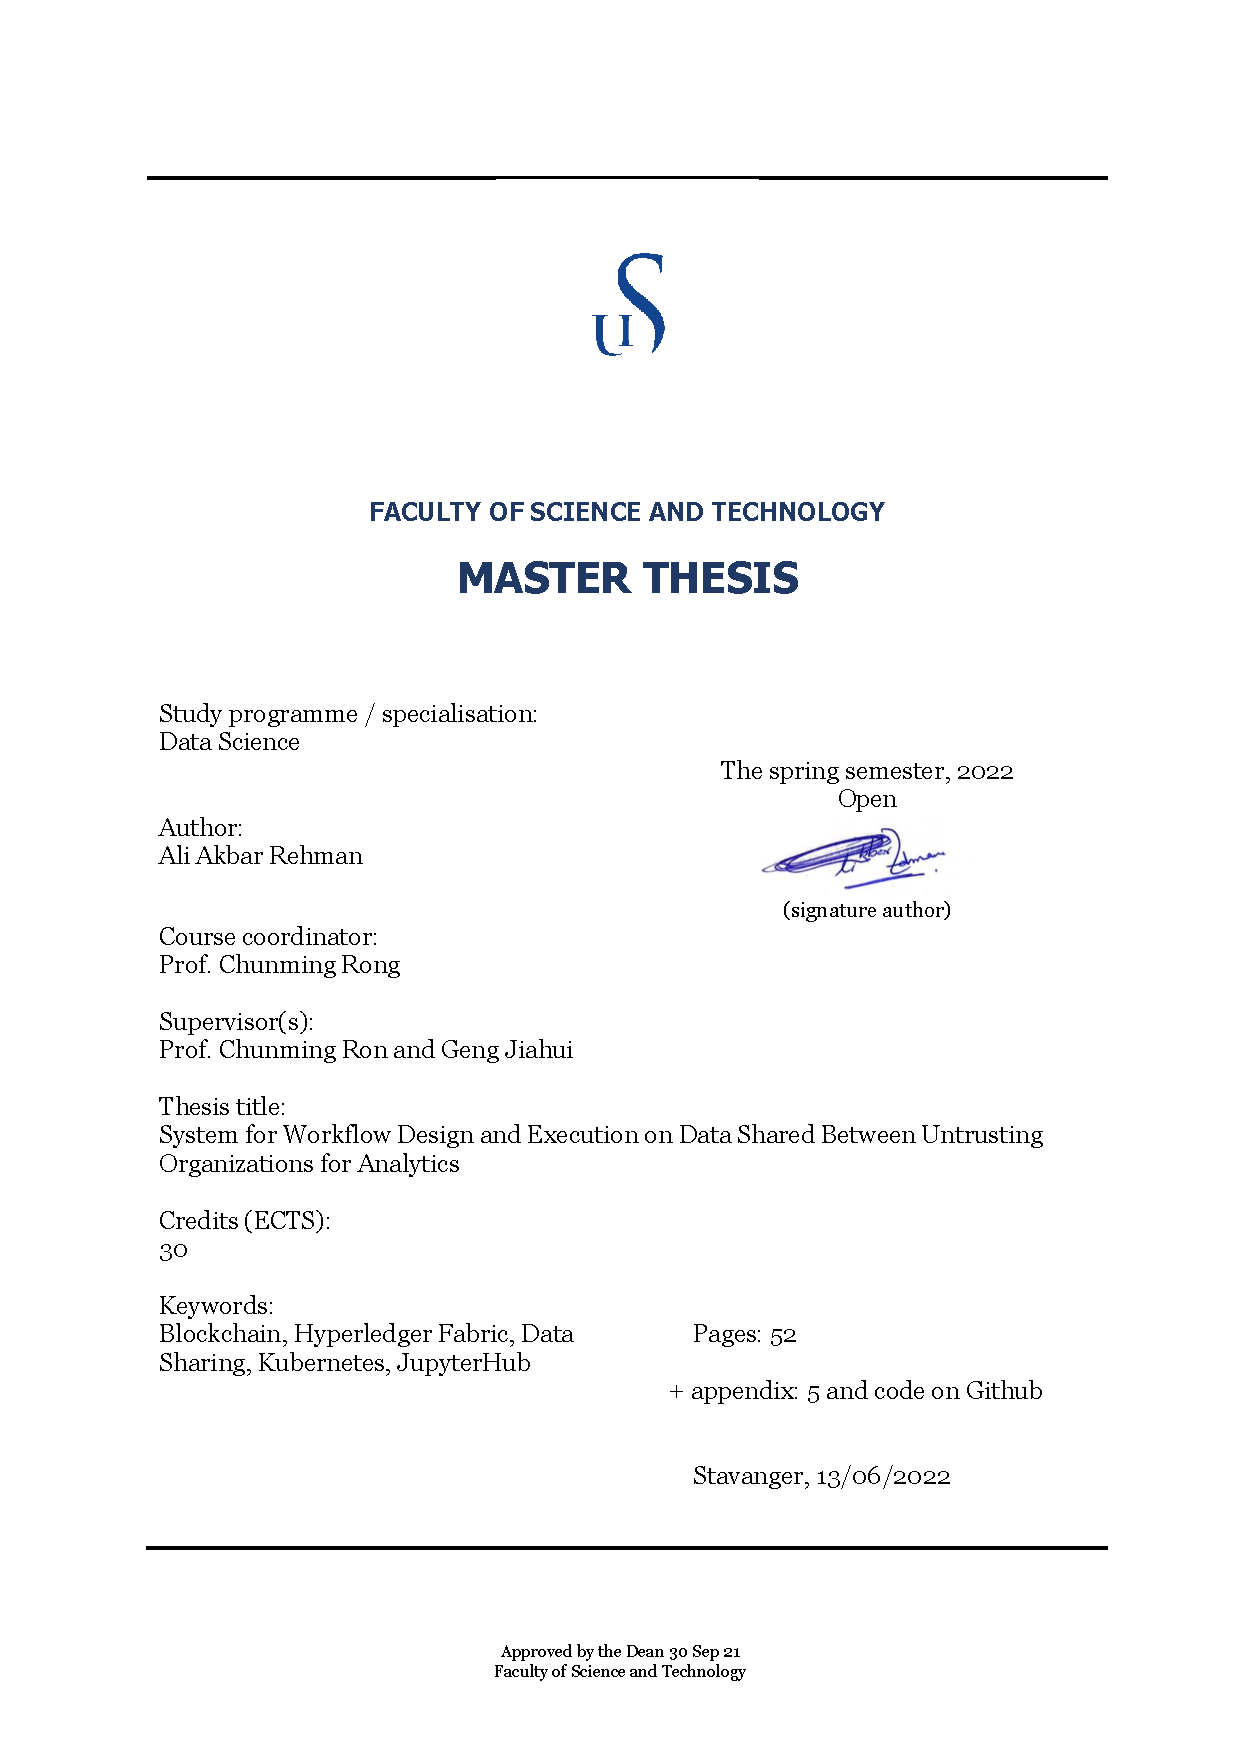
\includepdf{front-page}
\end{titlepage}
\uiscover{4}                  % pick color scheme 1-9
\frontmatter
\pagestyle{empty}
\declaration
%!TEX root = ../thesis.tex

\topskip0pt
\vspace*{\fill}

% Now comes the "Funny Quote", written in italics
{\Large\textit{``Learn patterns not technologies.''}}

\begin{flushright}
-- Unknown
\end{flushright}

\vspace*{\fill}

%!TEX root = ../thesis.tex

\abstract

Performance of complex analytics \& AI algorithms typically involves large amounts of data. The data may originate from multiple sources and is typically compiled and moved to a central location before it can be consumed by the algorithms, making this approach impractical for untrusting organizations interested to share analytics and results but not risking the exposure of the dataset in its entirety. Current approaches to support such a scenario for data consumption is to move the computation closer to the data instead of the other way around. But that involves writing code for distributed file systems like Hadoop File System (HDFS), which demands professional expertise in writing Map-Reduce jobs and parallel code design patterns. In this thesis, we demonstrate a proof of concept allowing organizations to share their datasets for consumption by inter-organizational workflows without exposing the data itself and avoiding distributed programming expertise. We propose an approach using Hyperledger Fabric for untrusting entities to advertise their datasets for consumption by other organizations without demanding extensive knowledge of writing distributed code, and all this without ever exposing the data itself to the user. Hence the analytics can be run on the data while maintaining ownership. A permissioned blockchain network is established using Hyperledger Fabric and organizations can join the mentioned consortium. A JupyterHub server is hosted on a Kubernetes cluster that services users with a Jupyter instance where users can explore the datasets available through our custom extension, write code and construct workflows running the algorithms on the datasets. The required datasets are consumed as persistent volumes when running the workflow; only exposing the data to the job requiring it. To ensure the privacy of sensitive information committed to the blockchain, organizations encrypt the sensitive information with keys that are internal to the organization.
%!TEX root = ../thesis.tex

\acknowledgements
For Kausar, my mother, a fountain of benevolence and composure. 

\noindent And Maqsood, my father, whose persistence and perseverance are what made it all possible.

\noindent A bout of gratitude is due to my supervisors Prof. Chunming Rong and Jiahui Geng for their support, guidance and ideas with writing this thesis.

\noindent A thankful nod to my colleagues and friends at work would not be remiss.

\noindent And everything to my tenacious brother, Osama, for who I am today.

\tableofcontents

% \input{frontmatter/abbrev}
% \input{frontmatter/symbols}

%-----------------------------------------------------------------
\mainmatter	  % Begin normal, numeric (1,2,3...) page numbering

% Include the chapters of the thesis, as separate files
% Just uncomment the lines as you write the chapters

%!TEX root = ../thesis.tex

\chapter{Introduction}
\label{ch:intro}
\section{Background and Motivation}
The most important asset a company possesses in this day and age is its data and with increasing volume and awareness the challenges around data storage, security, and consumption are also growing exponentially. Some organizations either have already shifted towards a cloud or hybrid architecture and some are in the process of this shift. The move to the cloud offers a flexible and robust solution for data storage as well as access control to the data through some kind of Role-Based Access Control (RBAC).

\bigskip
Many organizations, often competitors, possess datasets with similar information. These organizations may be interested in sharing insights from their data but are reluctant to expose their data and transfer ownership to others. The goal of such knowledge sharing would be to drive the research of the entire industry but concerns over data privacy and ownership hinder such collaboration.

\bigskip
The traditional approach towards complex analytical algorithms on some datasets involve transferring data, which may be originating from several sources, close to the compute resources, and then running the algorithms or training an AI model. But the approach becomes impractical when multiple organizations become involved and data sharing becomes complicated owing to regulations and privacy.

\bigskip
An approach garnering more and more focus is to move the computation closer to the data residence; solving most of the storage and security concerns. One concern, however, would be to develop the expertise in writing distributed code which could be expensive and time-consuming.

\bigskip
We propose a solution allowing orchestration of complex workflows where each job in the workflow consumes some data from one or multiple sources and results from individual jobs can be compiled when the workflow finishes. Such a design would allow organizations to share their data for consumption by algorithms while still maintaining the ownership of the data. And also eliminating the need to invest heavily into developing knowledge of writing distributed algorithms for utilization of data from multiple sources.


\section{Objectives}
The aim of this thesis project is to develop a proof of concept that will enable untrusting organizations to share their datasets while maintaining ownership and access control over the data. The system would allow users to write code and complex workflows to consume datasets from multiple sources without exposing the data itself to the users. The integration of this thesis with \cite{nft-thesis}, in the future, will help in proving ownership of datasets and computed results as Non-Fungible Tokens.

\begin{figure}
    \centering
    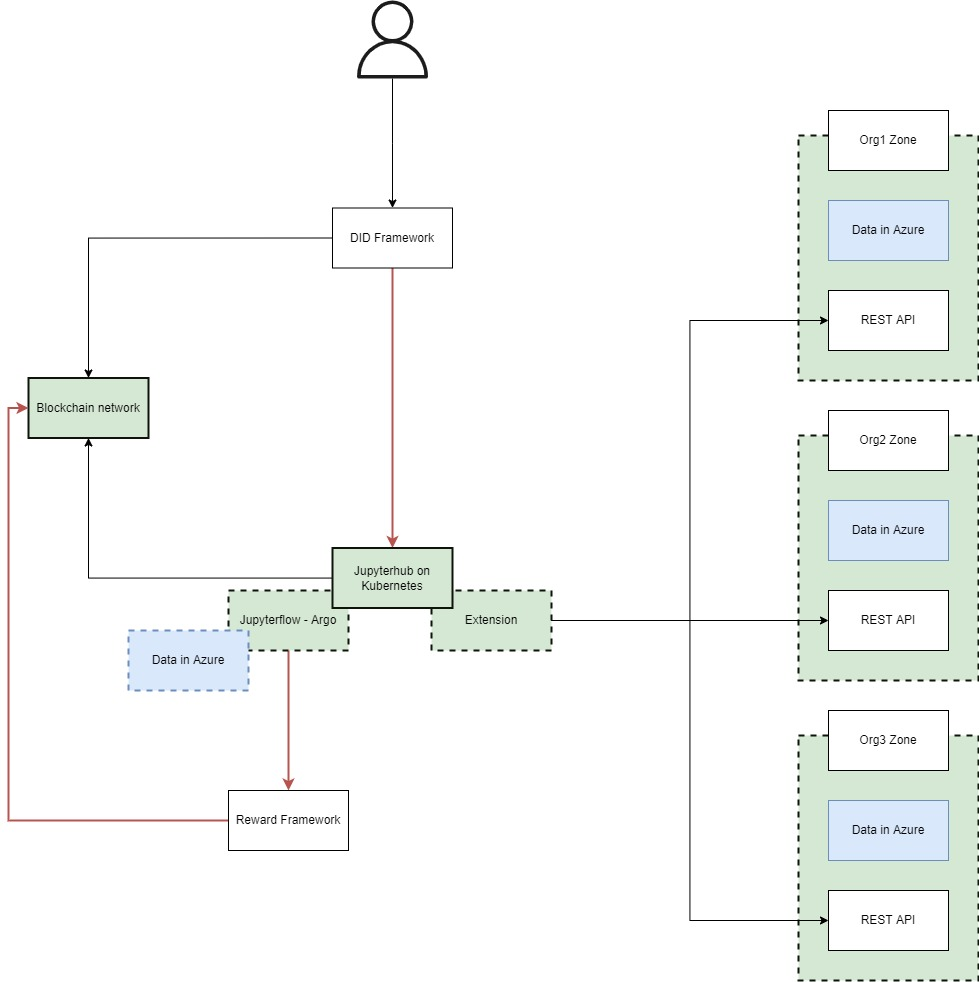
\includegraphics[width=14cm,keepaspectratio]{photos/Overview.jpg}
    \caption{Architecture of the overarching MVP that this thesis is a part of and the scope of the thesis}
    \label{fig:overview}
\end{figure}

\bigskip
The overarching Minimum Viable Product (this thesis in integration with Distributed Identity - DID and Data \& Results as NFTs) will allow for workflow design and development with access control of the entire system through DID and incentivization for contribution to the consortium through NFTs. The figure \ref{fig:overview} illustrates the architecture of the complete MVP. However, the scope of this thesis is highlighted by the green portions and is solely focused on the system for workflow design and data consumption. The DID and Reward Framework along with integrations highlighted in red fall outside the scope of this thesis.

\bigskip
The scope of this project comprises of following parts:
\begin{itemize}
    \item Establishing a blockchain network for containing meta-data of available datasets and a log of lease history of the data along with the chain code for committing the transaction to the ledger. The blockchain is constructed on Hyperledger Fabric.
    \item A REST API for keeping track of encryption keys in a MySQL Database and invoking the chain-code for respective requests.
    \item JupyterHub on a Kubernetes cluster where each organization can contribute nodes that will host Jupyter notebooks for users and act as an orchestrator for the entire system allowing design and execution for the workflows.
    \item An extension for JupyterHub that the users can utilize to explore and start work with a dataset.
    \item Extending JupyterFlow to mount Persistent Volumes on Kubernetes, create Persistent Volume Claims and trigger Argo Workflows on the cluster to run the user's code in a containerized form.
\end{itemize}

\section{Approach and Contributions}
The first component of our proposed system is to set up a blockchain network in Hyperledger where metadata of the datasets will be hosted. The idea behind using a blockchain is to enable organizations complete control over the information without trusting a third party as the maintainer of the system. The ledger keeps a track of all the datasets available from different organizations and a ledger of which organizations are using or have used the data. And the chaincode that could read and modify the state of the ledger. 

\bigskip
The next component is a REST API acting as the gateway between the blockchain and JupyterHub. We develop the API that responds to calls from the JupyterHub, does the validations on the requests, and invokes the corresponding chaincode. The API also stores and keeps track of the keys used to encrypt the sensitive information before committing to the blockchain. This API is going to be internal to the organization to keep the security of the keys integral.

\bigskip
The next key to the solution is the development of a custom Data Explorer extension for JupyterHub that will be interacting with the REST API and will be the interface for exploring and leasing the datasets as well as some admin operations for the maintenance of datasets. In this thesis the admin portion is visible to all however the integration with DID will enable fine-grain access control over the system. On triggering the lease of a dataset, a transaction is submitted to the blockchain, then a folder structure of the data is created in the user's JupyterHub environment to allow them to write code for the dataset and finally make the metadata ready for JupyterFlow to use by reading un-encrypted information vital for mounting the dataset on Kubernetes.

\bigskip
Finally, we fork and further develop the JupyterFlow \footnote{\url{https://github.com/hongkunyoo/jupyterflow}} to add the functionality enabling the mounting of data as persistent volumes in Kubernetes. The data can either be from a node in the Kubernetes cluster that the organization owns or from an Azure Fileshare. JupyterFlow then reads the information from the extension and creates persistent volume and persistent volume claims, generates an Argo workflow from the provided workflow YAML written by the user, and triggers the workflow to run.

\bigskip
Additionally, during the setup phase, we create a Kubernetes service account and set the token in the docker image where we also install the data explorer extension, our custom JupyterFlow, and some other dependencies. This docker image is used to spin up instances of Jupyter whenever a user logs in to the JupyterHub.

\section{Outline}

\subsection{Chapter 2 - Related Work}
This chapter presents some of the related work for this thesis and discusses the differences in our approach in comparison to the previous research and inspirations for some of the ideas in our thesis.

\subsection{Chapter 3 - Background}
In chapter three we present some background knowledge about the tools and technologies we have chosen for the development of our solution and discuss the reasoning behind the tools we have chosen.

\subsection{Chapter 4 - Approach}
In this chapter, we present and discuss our approach to developing the solution. We describe in detail how we use the different technologies and discuss the architecture of the proposed system. 

\subsection{Chapter 5 - Experiment and Demo}
Here we demonstrate how we have set up the test environment and the experiments we conducted on our system.

\subsection{Chapter 6 - Conclusions and Future Work}
Finally, we conclude our work, summarize the project and discuss the future directions for the project.
%!TEX root = ../thesis.tex

\chapter{Related Work}
\label{ch:related}
The traditional architecture of applications forces the participating users to trust a central authority. Such an architecture is proving to be outdated as we continue to realize the importance of our data. \cite{p2p-bitcoin} Proposed a system employing the blockchain technology to build a currency called Bitcoin that is maintained on a completely distributed ledger between untrusting parties. The paper highlights the algorithm to update the ledger without inserting malicious transactions. The paper proved that blockchain could be employed to maintain a central ledger without the need for a central authority. And the ledger records a tamper-proof history of transactions continuously.

\bigskip
Some of the most important services today are seemingly offered free of cost. However, the cost of these services is our personal data, and to use those indispensable services we are forced to rely on third-party organizations. This is the entire idea behind distributed apps and Web3.0 as discussed in detail here \cite{web3.0}. Web3.0 employs the concept behind the blockchain to develop completely distributed applications allowing complete freedom and Independence from third-party corporations.

\bigskip
Since 2008 when Bitcoin first came out as the first application of the blockchain concept, Web3.0 has been gaining continuous momentum. IBM and the Linux foundation developed \cite{ibm-hyperledger} Hyperledger Fabric, a private-permissioned blockchain to facilitate distributed application development between enterprise organizations. In \cite{x-org-workflow}, researchers propose a system to improve the current process of funds transfer between banks and parties from different countries for trading. The process usually takes days or weeks. The proposed system, however, developed using Hyperledger, automates a lot of the processes using smart contracts and reduces the time drastically. The research suggests a prototype based on blockchain to provide and enforce a workflow ensuring valid transactions between banks. 

\bigskip
\cite{collab-bw-adversaries} Explores the use of blockchain to enforce adversary parties to adhere to a predefined workflow. They however used the Ethereum blockchain providing a permissionless and public platform whereas we will be implementing our solution on Hyperledger to avoid using a public blockchain and only allow permissioned entities to join and keep the data private among organizations with a common interest.

\bigskip
Blockchain can provide a tamper-proof, central ledger without the need for a central authority. Mainly due to the fact that each block is vetted before addition but once added becomes a permanent part of the chain. This leads to complications when it comes to ownership of data and when the entity might want to remove its data. \cite{gdpr-compliant} Discusses among other things the very same idea to make the blockchain GDPR compliant so that once the data has served its purpose it can be purged. The proposed solution uses off-chain technology for each organization to maintain a set of encryption keys and only commit encrypted data to the chain. And once the encryption key is destroyed the on-chain data becomes useless. We employ a similar solution to share and maintain sensitive data on-chain. We employ the same technology to allow organizations to share the datasets and avoid committing any sensitive information to the blockchain.

\bigskip
In \cite{totem} and \cite{secure-computed-blockchain}, rather than compiling the datasets and running algorithms, the authors discuss the approach of dockerizing the code and running the containers on machines hosting the data. So the computation is moved to the place of residence of data rather than the other way around resulting in a solution where the data is not exposed to the user for computation. The system takes Map-Reduce code as input from the user and triggers them to run on the system hosting the data. Their proposed architecture makes use of a ledger in the Hyperledger Fabric network for governing access to remote resources and Hadoop for running Map-Reduce jobs on the system hosting the data.

\bigskip
The paper proposes a concept similar to that of Ethereum gas to constrain malicious users from running malicious code in the system. The users will obtain a fixed totem value that will gradually be used as the code is running. Running out of totem value revokes the user's privileges to execute code. Our approach slightly differs from the TOTEM architecture in that Organizations can use their current or cloud for storing data as long as they contribute nodes to the Kubernetes cluster they can join the consortium. The users do not have to develop the expertise to write Map-Reduce jobs and can use any language and design patterns they prefer as long as it can work on a Jupyter instance. The datasets will be moved across the network introducing the network overhead as compared to \cite{secure-computed-blockchain} but removing the complexity of writing distributed code. And the end goal of the systems is the same, some code is executed on the dataset but the user never gets to see the data itself, and ownership of the data continues to belong to the owning organization. And our recommendation to prevent users from writing code that simply copies over the data or to prevent them from misusing the system is to later introduce the step where the request to run some code would be reviewed and approved by the owning organizations hence preventing malicious code from running.

\bigskip
\cite{jupyterflow} Presents a solution to construct and run workflows as a set of multiple jobs. Each job is a command to run on a pod and we can define dependencies between the jobs as Directed Acyclic Graphs (DAG). It takes as input a \lstinline{workflow.yaml} file describing the jobs and their dependencies, converts it into an Argo Workflow, and runs it on the Kubernetes cluster hence introducing the requirement that the JupyterHub setup on Kubernetes only can run JupyterFlow. Our contribution takes the JupyterFlow plugin a step further. We develop and integrate the capability of creating Persistent Volumes and using Persistent Volume Claims in generated Argo workflows to mount datasets from different sources for the jobs that need the data. We will look into the example workflow and implementation details in Chapter 4. \ref{lst:basic-jflow} Shows a simple \lstinline{workflow.yaml} file that JupyterFlow can consume currently.

\begin{lstlisting}[caption={Example JupyterFlow workflow.yaml file having 5 jobs, from JupyterFlow official examples},label={lst:basic-jflow}]
jobs:
- bash hello.sh world
- bash hello.sh bob
- bash hello.sh foo
- ls
- echo 'jupyterflow is the best!'

dags:
- 1 >> 4
- 2 >> 4
- 3 >> 4
- 4 >> 5
\end{lstlisting}

%!TEX root = ../thesis.tex

\chapter{Background - Tools and Technologies}
\label{ch:background}

\section{Blockchain}
Blockchain \cite{p2p-bitcoin} serves as a ledger between untrusting parties. All the untrusting parties start participating in the peer-to-peer (p2p) network as peers and the algorithm allows for direct transactions to take place between the participating parties. Eliminating the need for a central authority maintaining the transactions altogether. All the transactions are vetted to be valid and non-malicious before being added to a block and becoming a permanent part of the chain. Once a block has been admitted into the chain, it can never be removed from the ledger. 

\bigskip
The validation of whether to add a block to the chain is done through a consensus algorithm. There is a choice of consensus algorithms dictating how a transaction is accepted into the chain. Over time several consensus algorithms have been developed each with its pros and cons. Normally it is a trade-off between speed and security, but the algorithms are being improved upon to come up with a consensus algorithm that is both fast and safe. Bitcoin uses an algorithm called proof-of-work as a consensus, which ensures the miner has done enough amount of work to add the block to the chain and that to change it the same amount of work would go into mining every subsequent block. It has its shortcomings. Proof of Work is slow and energy inefficient, Ethereum is proposing to move to a proof-of-stake algorithm for consensus, where the network holds on to the stake of the miner till it is verified that the blocks added are valid. The takeaway point here is that the consensus algorithm is one of the core things setting apart a blockchain from other blockchain networks. As we will discuss later, Hyperledger uses a consensus algorithm where the transactions have to be signed by the peers according to a policy before being added to the chain, the benefit of having a private chain with identified entities.

\bigskip
The distributed ledger technology is a lot older than Bitcoin. \cite{blind-signatures} and \cite{secure-names} are papers from the 90's discussing the establishment of a distributed ledger in a peer-to-peer network. Bitcoin was the practical implementation of the algorithm as a crypto-currency in 2008 by researcher(s) under the assumed name of Satoshi Nakamoto. As discussed earlier, Bitcoin uses something known as proof-of-work as the consensus algorithm where each transaction is timestamped and its hash included in the chain ensuring that changing a transaction demands all the transactions afterward need to be recomputed. Since this hashing is a computationally expensive process, as long as a majority of the peers in the network are not conspiring for an attack (The probability of which happening is very low), the longest chain can be accepted as an un-tampered ledger.

\bigskip
The main characteristics, as apparent from \cite{p2p-bitcoin}, of the blockchain network and a distributed ledger in general are:
\begin{itemize}
    \item \textbf{Distributed:} The main building block of a blockchain is a Node. A node can be thought of as a single machine that is part of the network. Once a blockchain network is started, nodes can join the network and start participating. Every node keeps a copy of the ledger and every suggested transaction is validated by comparing each node before being committed to the chain. The validation process involves the comparison of hashes from previous blocks \& suggested hashes. This distributed nature makes blockchain resilient from takeover since a corrupted block will be immediately recognized and discarded.
    \item \textbf{Secured:} Whenever a new transaction is to be added to the chain, a transaction is broadcasted to the entire network. Each node verifies if the transactions, about to be committed, are legitimate. If they are, the block is admitted to the chain, and every node is made aware of the update else the block is discarded. Since no authority is in charge of the majority of the nodes the network cannot be hijacked and ensuring the ledger is secure against attacks.
    \item \textbf{Smart Contracts:} Smart contracts are a supplement to the blockchain technology because they were added as a functionality later on. They are small pieces of code that reside on the nodes alongside ledger copies and can be invoked when interacting with the blockchain, in a way enforcing a contract. Smart contracts provide the flexibility to enforce contracts and since they are written in code they can be very diverse in the kind of operations they perform.
\end{itemize}

Before moving on to the specific technology we have opted for let us discuss a little about different types of the blockchain. There are two main types of a blockchain networks and which are permissionless \& permissioned networks. A permissionless blockchain network, also known as a public blockchain is one where anyone can choose to participate in the network. The crypto-currencies like Bitcoin, Ethereum, and countless others belong to this type of permissionless or public blockchain. And since anyone can participate it becomes harder or nearly impossible to identify and track users of the network. In contrast to permissionless blockchain networks, permissioned blockchains are a new concept quickly catching on. Instead of a completely public network, permissioned blockchains allow the establishment of a network where users can be identified and need to be enrolled before being allowed into the network. This type of blockchain is best suited for the development of distributed applications or a distributed ledger among organizations that need to collaborate but possess a certain distrust or competitiveness between them. In such a network each user is identified by a digital certificate and users are assigned permissions by administrators. Thus giving administrators control over the actions the users are allowed to perform in the network. This gives another layer of security to private blockchains in comparison to public blockchains. Because of these principles, permissioned blockchains are getting increasingly popular with enterprise organizations.

\subsection{Hyperledger Fabric}
Hyperledger Fabric \cite{ibm-hyperledger}, is an Open Source project started by the Linux Foundation. It provides the tools to set up a private \& permissioned blockchain network among parties. It has been designed from the ground up to be modular where the components are plug-n-play to support a wide area of scenarios and enterprises. Once a network has been established, Organizations can join channels which is the Hyperledger terminology of a blockchain. Each channel can have its ledger and smart contracts. And because of this setup Hyperledger can support multiple ledgers between the participating organizations. Another big reason to opt for Hyperledger Fabric is the fact that it supports smart contracts (Chaincode in Hyperledger Terminology) in multiple programming languages such as Java, Go, or NodeJS. Listed below are the main components of the Hyperledger Fabric:
\begin{itemize}
    \item \textbf{Channel:} A channel can be thought of as a dedicated communication channel between organizations in a network. Organizations with similar interests come together as a group and decide to set up a blockchain network. They formulate an application channel; there is a system channel that Hyperledger uses internally for the maintenance of the network. After a channel has been created nodes can start to join and participate in this channel. And each node that joins the channel gets a copy of the ledger. And each channel supports a versioning setup for smart contracts. As discussed in the \cite{fabric-network} Hyperledger Docs, the ledger is physically hosted on the peer nodes but logically hosted on the channel. Policies regarding endorsement of the transactions are set up when starting the channel as well. Each channel will have several peer nodes and one orderer node; which acts as the orchestrator between the peer nodes. After a transaction has been signed/endorsed by the required peers (as dictated by the policy), the orderer will distribute the block containing the transaction to the peers to be added to the ledger.
    \item \textbf{Membership Service Provider:} Hyperledger being a permissioned network needs some infrastructure to identify users before allowing them to interact with the blockchain. This is where a membership service provider (MSP) comes in. Each entity participating in the network requires a key and a certificate according to the Public Key Infrastructure (PKI) from Certified Authority (CA) and the certificates are used to enroll the entity with the MSP. Afterward, the MSP can identify the entity and the permissions it possesses. To understand an MSP consider a scenario to add a new user to an organization participating on the network, the scenario starts by getting a Public-Private Key pair from a Certified Authority, and enrolling the user in the organization using the MSP; this is the step user has it's certificate added and linked to a role in the organization by the MSP.
    \item \textbf{Chaincode:} Chaincode is the Hyperledger terminology for a smart contract. It is the piece of code that dictates the interactions with the ledger. Instead of getting the ledger directly, the chaincode is invoked which in turn performs operations involving the ledger. In simple words, chaincode is the business logic surrounding a blockchain ledger. Similar to the ledger, chaincode is logically hosted on a channel while physically hosted on peers. As discussed earlier, Hyperledger supports chaincode written in several languages like Java, NodeJS, and Go, making it easily adaptable in the industry.
\end{itemize}

To better understand how all these different components in Hyperledger Fabric work and how the Fabric blockchain network is constructed, we use the example of a sample network from Hyperledger Documentation \ref{fig:hyperledger-sample-network}. In  \footnote{\url{https://hyperledger-fabric.readthedocs.io/en/latest/network/network.html}} We have three organizations R1, R2, and R3 wanting to establish a consortium CC1. CC1 has the policies and role definitions for organizations \& their individual users along with endorsement policies for transactions. CA0, CA1, and CA2 are the certified authorities that organizations R0, R1, and R2 use respectively. They are responsible for generating identities under the Public Key Infrastructure that will be registered by the Membership Service Provider. R1 and R2 join the logical communication channel C1 with Peers P1 and P2 while R0 only contributes an orderer node. Each node hosts a copy of the ledger while the peer nodes also host Smart Contracts or chain-code S5. And lastly R1 and R2 own Applications A1 and A2 that they use to interact with the network.

\begin{figure}
    \centering
    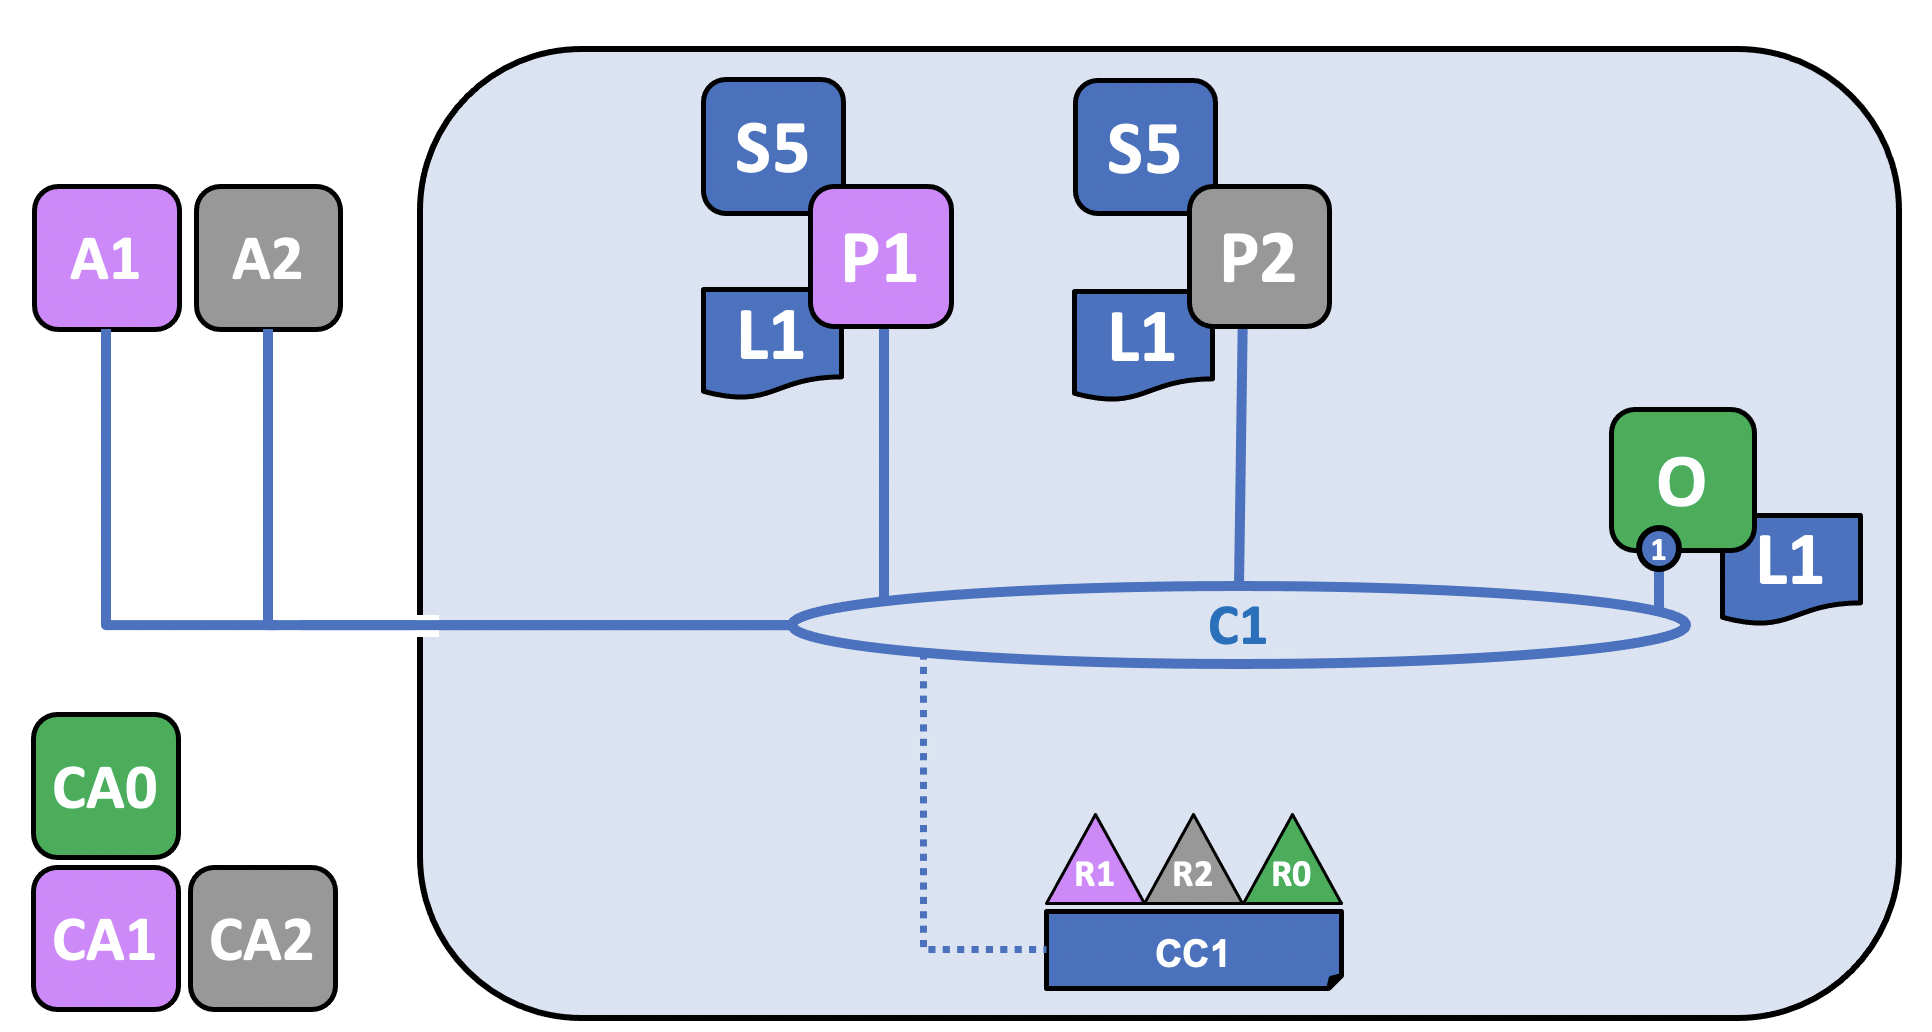
\includegraphics[width=12cm,height=12cm,keepaspectratio]{photos/network.diagram.1.png}
    \caption{A sample blockchain network between two organizations and an orderer organization, one channel and smart contracts.}
    \label{fig:hyperledger-sample-network}
\end{figure}

\bigskip
The flexibility that Hyperledger offers, in terms of setting up a private blockchain network with a modular architecture makes it the first choice for enterprise use. Pluggable CA and MSP framework, consensus policies along with the opportunity to set up complex private channel structures on the same p2p network and smart contracts in several mainstream programming languages, make it fit for a wide spectrum of scenarios. You can find several systems already in production developed using Hyperledger and a number of its sub-modules \footnote{\url{https://www.hyperledger.org/learn/blockchain-showcase}}. These are the reasons we decided to use blockchain and Hyperledger to maintain a list of shared datasets where organizations are in control without trusting a third party to maintain the system.

\section{Kubernetes}
Kubernetes or Kubernetes is an open-source tool developed by Google for orchestration, scaling, and management of containerized applications. Kubernetes operates in a cluster, which is a collection of virtual machines (VMs) overlooked by a master node. The master node is only an API server for Kubernetes admins to interact with the Kubernetes admin client instead of managing each VM separately.

\bigskip
Several cloud providers provide a managed Kubernetes cluster as Platform As A Service (PAAS) where the cloud providers are responsible for maintaining the underlying infrastructure. With implementation details like VM management and configuration of the Kubernetes cluster are kept hidden from the users and users can start using Kubernetes right out of the box. However, such a setup is not feasible for our use case. We need to set up and maintain a Kubernetes cluster ourselves so that organizations can join and leave the cluster at will and can also join nodes where data is hosted on the node itself.

\subsection{Containers}
Before going into Kubernetes, we can briefly present a background regarding container technology. Containers are the evolution of virtualization technology. Unlike virtual machines where a complete system including the physical infrastructure along with a kernel and Operating System (OS) is virtualized, containers only virtualize the OS, and off-loading the maintenance of the hardware to the host OS and sharing the kernel results in computationally very cheap virtualization technology. Containers wrap around a bare-bones OS and package all the dependencies inside an Image that can be used to spin up a replica of an application/system anywhere on any machine. And containers run completely isolated from the host system as an extra security layer so as not to affect the host machine.

\bigskip
The biggest service for container technology is Docker. Docker is available for all major operating systems and architectures. Applications can be containerized using a simple \lstinline{Dockerfile}. Docker uses the \lstinline{Dockerfile} to create an image that can then be used to spin up containers anywhere, with the same parameters, in seconds compared to minutes of virtual machine allocation and start-ups. 

\bigskip
Docker-Compose is a supplement to the bare bones docker system. Docker-compose allows packaging and running multiple containers as services; that might be dependent on each other; with a single command. Yet Another Markup Language (YAML) file can be used to describe different containers, their environment, volumes, and networks and the running of a single command spins up all the dependent services with the parameters specified. We use docker and docker-compose not only to spin up not only a test blockchain network using Hyperledger but also to allocate isolated environments for each user that logs in to use Jupyterhub.

\bigskip
Coming back to Kubernetes offerings and why we decided to use Kubernetes in our system. Kubernetes offers features such as health checks of running containers and restarts in case of node or container failures. Supports the scaling up of applications depending on the resource demand and load balancing between horizontally scaled services or scaling down in case demand goes down. Provides several, easy plug-in storage options so applications do not care about the storage infrastructure and Kubernetes can handle that whether a Cloud (Azure, AWS, or GCP) storage solution is used or a node-local one or even a network shared file system.

\bigskip
Because of the auto-scaling and optimized utilization of the resources, Kubernetes as a tool is very useful and interesting for data scientists, who frequently need to run resource-heavy simulations or analytics on often gigantic data sets. However Kubernetes has a steep learning curve and in practicality serves more use cases from a software engineer's perspective than a data scientist, even though it can be an extremely useful tool for running compute-heavy workloads. 

\bigskip
The first reason we incorporate Kubernetes into our system is the obvious benefit Kubernetes presents when running compute-heavy workloads. Also, we want to allow organizations to contribute the compute resources in addition to sharing datasets. Secondly, as discussed earlier Kubernetes offers a plug-n-play solution for using data from several sources and storage systems. We intend to leverage this feature to support a wide number of storage systems, allowing organizations flexibility to use any storage system and not causing hindrance for organizations to participate in our system. In the proof of concept we are only using Azure but because of Kubernetes wide storage support can be easily extended. Next up we intend to make use of JupyterHub, JupyterFlow, and Argo Workflow for giving users an environment to write code, construct workflows and trigger them instead of developing the environment ourselves and hence the choice to use Kubernetes. And as discussed in future work can help give weightage to the computed results, to the organizations contributing more resources towards computation as well as datasets, and then incentivize when those results are utilized or even sell their stake in the results.

\subsection{Jupyterhub}
Project Jupyter started as a simple interface providing a Jupyter notebook that provides runnable modules within itself and thus supports interactive programming. And in addition to the interactive programming support, Jupyter also provides support for running kernel commands directly from the notebook. It is one of the most widely used Integrated Development Environment (IDE) for Python and data science. Jupyter is a set of open-sourced software and standards for interactive programming across several languages but is found most used in Python settings. The notebook is still the most basic block of a Jupyter environment but it has developed into a much more diverse set of tools. We will take a look a JupyterHub in this section.

\bigskip
JupyterHub is an enterprise solution for big companies and research labs to host multi-user Jupyter environments on a server. It runs on a central server or a Kubernetes cluster and can spawn multiple instances of single-user notebook servers and hence providing each user with an isolated environment (to avoid conflicting processes and security of the underlying infrastructure). JupyterHub is designed to be containerized and Kubernetes friendly and thus can scale up and down depending on the number of users. It provides a pluggable authentication service to support several identity providers. Currently, it supports Privileged Access Management (PAM), Lightweight Directory Access Protocol (LDAP), and OAuthenticator out of the box and supports custom Authenticator Interface implementation implemented following OAuth standards. One of the projects alongside this thesis is to develop a Distributed Identity using blockchain and a custom Authenticator for JupyterHub. The integration with DID framework and using the custom authenticator falls out of the scope of this project. These all features combined make it a perfect tool for a consortium of organizations to serve users with a single-point solution for data analytics. 

\bigskip
Jupyter has grown from a single notebook to an array of tools and JupyterLab is the next generation of the Jupyter interface. JupyterLab is a completely new extensible interface for Jupyter. Unlike the classic notebook interface, JupyterLab is designed from the ground up to be a modular solution and a complete integrated environment with powerful tools like a file explorer, multiple programming language kernels and terminals, and editors with embedded debuggers. In addition to all this, JupyterLab allows the use and motivates the development of community-driven third-party extensions. We turn on the JupyterLab interface on JupyterHub and develop a custom extension to explore the datasets. All these features of JupyterHub and JupyterLab make it the ideal tool for the development of a workflow management system aimed at allowing organizations to collaborate.

\subsection{Argo Workflow}
Argo workflow is an open-source tool or Custom Resource Definition for Kubernetes that provides the ability to define complex workflows and can trigger them on Kubernetes. In Argo we can specify each job in the workflow as a collection of Docker images, volumes and environment variables and Argo can spin up the respective pods. Argo also provided the functionality to specify dependencies among workflow jobs as Directed A-cyclic Graphs (DAG) and takes care of triggering jobs in the order of our workflow, triggering parallel jobs together and waiting for dependant jobs to finish before triggering the next one.

\bigskip
After installing Argo Workflow, we can start writing YAML files for workflows that can be consumed by Argo to trigger pods on Kubernetes. Argo also exposes a web User Interface (UI) for users to see the workflows triggered, monitor them for errors and check logs, etc. Another useful feature of Argo is exit handlers, which enable the user to specify exit strategies in case of success or failure both, to clean up the resources that Argo was consuming. We have not managed to utilize this feature in this thesis but we discuss how it can be useful in future work \ref{ch:conclusion}.

\subsection{JupyterFlow}
As discussed earlier, the auto-scaling nature of Kubernetes and now tools like JupyterHub that run natively on Kubernetes, make it the ideal solution to run computationally heavy machine learning or statistical workflows on. However Kubernetes has a relatively steep learning curve and as data scientists, our energies need to be focused on data rather than configuring and working towards running our workflows on Kubernetes. Before we can run our workflows on Kubernetes we need to containerize our code along with any environment configurations. To allow data scientists to use Kubernetes to run their workflows without tinkering too much with Kubernetes we need an abstract tool that can handle Kubernetes configuration and configuration details on its own and allow us as a user to just run workflows. JupyterFlow \cite{jupyterflow} is this tool, distributed as a Package Installer for Python (PIP) package.

\bigskip
JupyterFlow is a tool that is logically built on top of JupyterHub on K8s and Argo Workflows. As discussed in the previous subsection Argo allows writing YAML workflows as custom Kubernetes objects and takes responsibility to trigger the respective pods in the order that workflow requires. JupyterFlow uses Argo and Kubernetes API under the hood and makes it even simple for us as data scientists to focus on data and not take on a role of a software engineer. It takes the image and environment that JupyterHub uses to spin up the Jupyter instance for the user and a very simplified YAML file and constructs an Argo workflow and then triggers it on the Kubernetes cluster.

\bigskip
The only limitation for JupyterFlow is that it only works on JupyterHub on Kubernetes. Since we already have chosen to use JupyterHub on Kubernetes as a platform for users to work on, JupyterFlow fits perfectly into our scenario and we can extend it to use custom volumes on each job while still maintaining the simplicity, that JupyterFlow brings.

\bigskip
JupyterFlow removes the overhead of containerizing the code and writing insanely complex Argo YAML files to run the complex workflows on a Kubernetes cluster. Since JupyterHub on Kubernetes can spawn up a separate single-user Jupyter instance for every user that logs in by using a pre-built docker image with all the dependencies installed and environment setup. As JupyterFlow runs on top of JupyterHub on K8s, it can use the Kubernetes API to get the image used for setting up the environment and fetch the volume details for the user's home directory. JupyterFlow can use these two details to containerize the environment without users' intervention. To pass the code the user has been working with inside the Jupyter server, it utilizes the shared storage solutions that JupyterHub on Kubernetes offers natively. Since each user gets their shared access storage so the code and files the user works with are already accessible to Kubernetes we only need to make it available to the workflow that Kubernetes is gonna run. After these details have been fetched, JupyterFlow uses a template of Argo workflows to compile the Argo workflow YAML file from the simple YAML file provided by the user. In this way, JupyterFlow removes the overhead of learning Kubernetes and writing complex workflow YAML files. It can take a simple YAML file \ref{lst:basic-jflow} and takes care of containerizing, creating Argo workflows from it, and triggering it on Kubernetes.

\section{Storage Solutions}
The last piece of the puzzle for our proof of concept is the storage solutions we can support to consume. Most organizations are moving their on-premise infrastructure to the cloud or a hybrid model. And cloud storage gives them the flexibility to store enormous amounts of data without the hassle of maintaining the infrastructure. Cloud Providers offload the responsibility and make the data highly available, scalable, and secure through Role-Based Access Control (RBAC). 

\bigskip
Kubernetes can support mounting volumes for containers from several storage sources. In this thesis, we develop the system to support Azure Fileshare and Storage on Kubernetes Nodes as the two available storage solutions. We opt for Microsoft's Azure platform owning to the huge presence in the Nordics and the great resources available. We make use of Azure Fileshare which organizations can use to store their data and when needed we can mount the Fileshare on the Kubernetes Cluster, may be residing in the same data center and using the data for analytics without giving up the ownership of the data itself to the consuming user. 

To summarize we have discussed in this section the technologies we have chosen to develop our proof of concept and why we have chosen the technologies. And a brief overview of what is the responsibility of each component. \ref{fig:component-jobs} highlights a visual representation of all the components involved in the system and what function each component serves in our architecture.

\begin{figure}
    \centering
    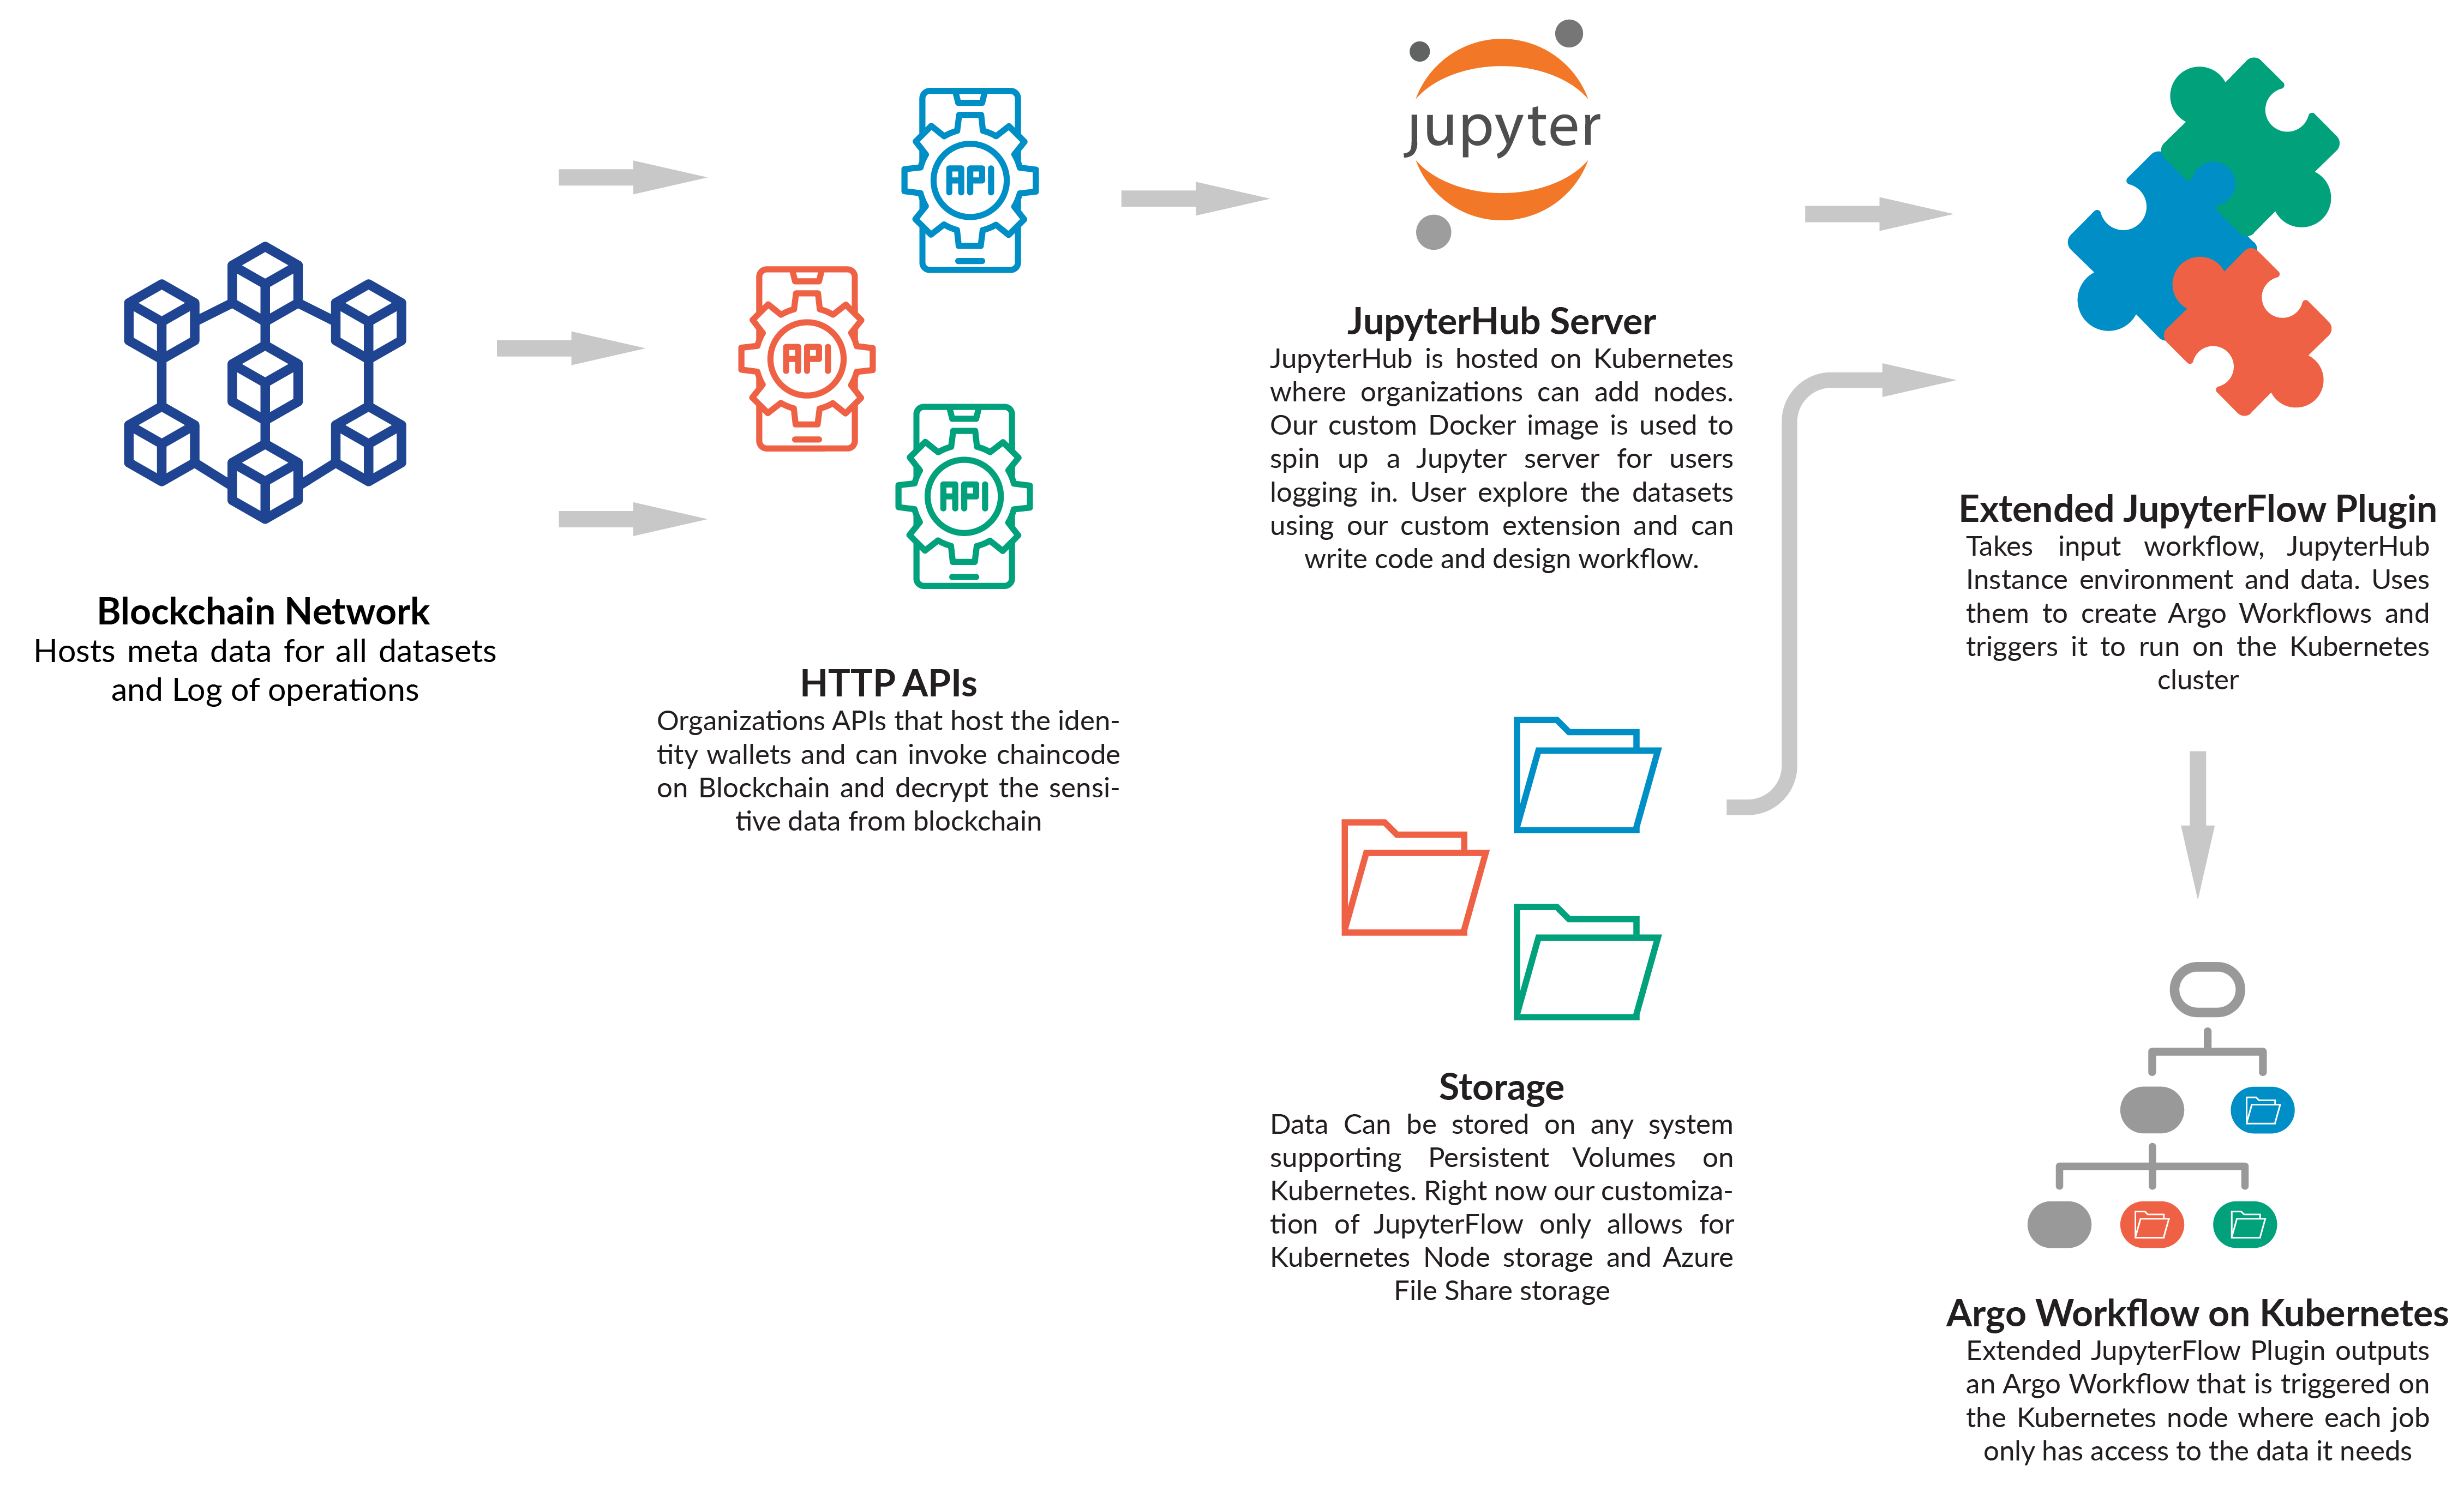
\includegraphics[width=14cm,keepaspectratio]{photos/overview.png}
    \caption{The tools and technologies discussed in background section and how they all integrate and work together in the proposed system.}
    \label{fig:component-jobs}
\end{figure}
%!TEX root = ../thesis.tex

\chapter{Approach}
\label{ch:approach}

\section{Introduction}
 In chapter 2 we discuss the object of the thesis, which is to design and develop the workflow that enables organizations to share their datasets for consumption by users from other organizations without exposing the dataset itself. And the system that we are trying to develop should allow users to write code without developing expertise to write distributed code like Hadoop's MapReduce Jobs.
 
 \bigskip
 This thesis is part of a bigger proof of concept that incorporates this system together with Distributed Identity Framework (DID) and authenticator for JupyterHub as well as integrating this with the NFT Framework for proving ownership and stake in data as well as results. The integration between the workflow and other parts of the final proof of concept does not fall under the scope of this thesis.
 
 \bigskip
 The overview of our approach is briefly demonstrated in \ref{fig:component-jobs}. We set up a Hyperledger network using docker-compose with three organizations and smart contracts/chaincode that will be invoked by a REST API. The REST API is an application that will be owned by the organization and can be made internal to the organization since it will be interacting and storing with the MySQL database to store keys for encryption/decryption of sensitive data before committing to the blockchain. However, as part of this proof of concept, we only create one instance of the API. As the next step, we set up a Kubernetes cluster and install Argo and JupyterHub on the cluster. The users can log in to this JupyterHub environment to use it as an IDE and explore the datasets available. We develop a custom extension for JupyterHub for navigating the datasets and develop JupyterFlow further to create Persistent Volumes, mount Persistent Volume Claims on Kubernetes, and create Argo Workflow from a template and trigger the workflow with those volumes mounted for jobs requiring the data.

\bigskip
Before delving into the details of the implementation we want to acknowledge that the work we present here is only a proof of concept and contains several loopholes and security vulnerabilities that need to be addressed in future work before this work can be considered to be production-ready. Moreover, we assume that one organization takes charge of initiating the consortium and that organizations agree to the policies and rules before joining in. Moreover, we acknowledge the system can be exploited very easily given that the secrets after reading from the blockchain are stored in a plain text hidden file and are only secure by obscurity. This can be improved later to stop the user from reading these sensitive values. Moreover, the details like user id and roles will be available from the Distributed Identity framework once integrated, which right now are input and any user can take the role of any other user.

\section{Proposed Solution \& How it Works}

\begin{figure}
    \centering
    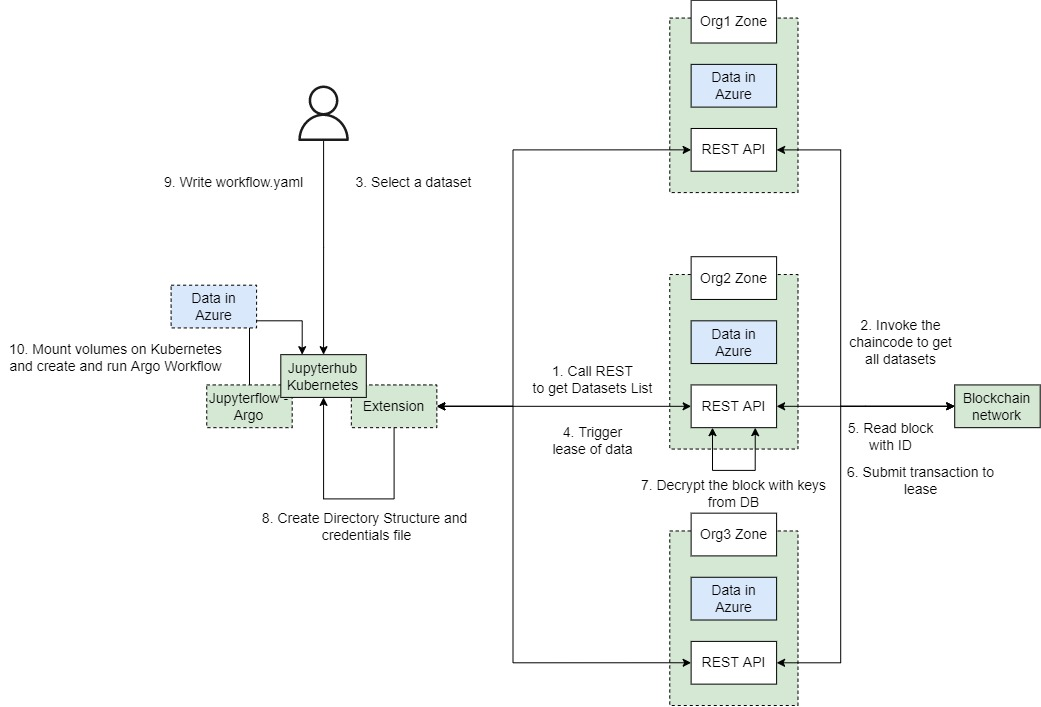
\includegraphics[width=14cm,keepaspectratio]{photos/how-it-works-2.jpg}
    \caption{Step by step process of the workflow of the information and instructions in the system.}
    \label{fig:how-it-works}
\end{figure}
Figure \ref{fig:how-it-works} highlights a step-by-step process of how the entire proof of concept works to consume datasets from multiple sources in a workflow without ever sharing the ownership and not allowing the user to even see the data.

\begin{enumerate}
    \item Read a list of all the datasets available from the Hyperledger Fabric network by calling the REST API that invokes the necessary chaincode.
    \item User selects one or more datasets to consume in jobs inside the workflow that will be triggered later.
    \item The extension triggers the lease endpoint in the REST API.
    \item The REST API invokes the chaincode that will submit the transaction to lease the data. If the data is free it will be leased else an error thrown.
    \item The chaincode to get the block using the ID is invoked. The REST API gets the decryption keys for the specific data block from the database and returns the decrypted data.
    \item Extension received a response from the API and creates a directory structure for the user to experiment with and write the code.
    \item Extension creates a hidden file with the credentials to mount the data as a persistent volume claim in Kubernetes.
    \item User writes a \lstinline{workflow.yaml}
    \item JupyterFlow creates a persistent volume on Kubernetes, creates a claim, and uses those claims for relevant jobs. Creates an Argo Workflow and triggers it.
    \item The Argo workflow runs and computes the results.
\end{enumerate}

\section{Implementation Details}
\subsection{Setting up Blockchain Network}
In the system we propose organizations will be storing metadata about their datasets on a blockchain to have full control of themselves and not a trusted third party that in traditional architecture will be maintaining the system. We will set up a blockchain network in Hyperledger Fabric with three organizations and one orderer organization. Each organization in the test network will contribute only a single peer node.

\bigskip
Since Hyperledger is a permissioned/private blockchain, every entity on the chain needs private keys and certificates following public key infrastructure issued by a certified authority to identify them. In a production scenario, each organization will have a different CA who will be responsible for providing certificates not only for the users but also for the peer nodes. In our test environment, we use the CA tools provided by Hyperledger designed and available specifically for test environments. We spin up docker containers for each organization and the identities of an admin, a user, and a peer are generated by the CA. We enroll them in the respective organizations as part of the setup process.

\bigskip
Hyperledger uses the identities to identify the participating entity and see if the policies allow the specific entity to perform the requested operation. Policies are rules that each organization sets up when joining a channel to specify who can perform which operations on the network. Consider the following policies that we have for UiS (One of our test organizations). For testing, we use the same policies for each organization. These policies can be configured in \lstinline{configtx.yaml} and each organization can write its own users' and peers' policies according to its internal structure.

\begin{lstlisting}[caption={Policies for UiS (one of our test organization). We use the same policies for other organizations as well.}]
Policies:
    Readers:
        Type: Signature
        Rule: "OR('UiSMSP.admin', 'UiSMSP.peer', 'UiSMSP.client')"
    Writers:
        Type: Signature
        Rule: "OR('UiSMSP.admin', 'UiSMSP.client')"
    Admins:
        Type: Signature
        Rule: "OR('UiSMSP.admin')"
    Endorsement:
        Type: Signature
        Rule: "OR('UiSMSP.peer')"
\end{lstlisting}

\bigskip
So we have four roles stating who can read, write, administer the organization (Add users, peers, etc.) and endorse transactions. And policies can use AND, OR and other binary operators to define rules for each role. Here we want to highlight also why participants need to be enrolled in the MSP because the network uses MSP to attach identities to their roles. As an example, once an entity is registered in the MSP either as an admin, peer (because chaincode runs with peers identity), or a user they are eligible to read from the ledger.

\bigskip
We have already seen the policies that dictate in a network and that they are specified in a \lstinline{configtx.yaml} file. \lstinline{configtx.yaml} hosts a few other configurations as well in addition to the policies. In this file, first, we define the organizations in the network with the name, location for identities, and policies for each organization. Also, keep in mind that organizations can later be added to the network. That is the reason we set up a network with two test organizations and add a third one later but we will discuss more on that in \ref{ch:eval}. Next, we configure the capabilities section which is left default since this section is internal to Hyperledger to dictate which features are available in the version being used. The application-level configuration and policies dictate how smart contracts are configured to behave and which organizations are allowed to endorse the addition of a new version of a chaincode or a new chaincode altogether on the channel. And finally, we have the profile configuration, stating the organizations that will be part of an application channel.

\bigskip
After the initial setup, we create similar configurations for the third organization and follow the same procedure to add it to the channel by creating identities and enrolling these identities with the MSP, and then adding them to the channel we created previously. The only difference is that the Majority of other organizations need to approve or endorse when adding a new organization as specified in the policies of the application channel when setting up the network.

\subsection{Chaincode}
Hyperledger applications can not read or update the ledger directly, rather they interface with the blockchain and the ledger through the chaincode. Chaincode is Hyperledger terminology for smart contracts and contains the business logic of the network whenever processing a transaction on the block. So chaincode is a vital part of any network.

\bigskip
As mentioned before, Hyperledger, unlike other blockchain frameworks provide the opportunity to write chaincode in languages like Go, Java, and NodeJS. We develop our chaincode in JavaScript. Chaincode needs to implement the Contract class provided by the fabric-contract-api package for Node. And each method in the class is auto-injected with context that allows it to read from the world state of the ledger and submit transactions to modify the ledger. The transactions then need to be endorsed by peers from other organizations as stated in the policies when setting up the channel. These methods are then invoked by external, off-chain applications in our case the REST API.

\bigskip
Each block on the chain is metadata about a dataset that an organization wants to share. And apart from the organization having complete control over who can access this on the blockchain, this being a ledger we are continuously getting an immutable log of who and when updated the block and also who the dataset was leased to. As part of designing the workflow that allows for the consumption of data, a Create, Read, Update and Delete (CRUD) chaincode would suffice. In addition to the update chaincode, we have another chaincode that only leases a dataset from one organization to another after validating that the dataset is not in use. 

\bigskip
Here are the outlined steps needed to add chaincode to the channel and are implemented in \lstinline{deploy.sh}. Also mentioned are the commands for each step.

\begin{itemize}
    \item \textbf{Packaging} The first step is to package the chaincode into a tar archive. If same chaincode is going to be running for every organization then only one organization can complete this step and share the packaged code off-channel. 
    \begin{lstlisting}[language=bash]
        peer lifecycle chaincode package data-chaincode.tar.gz --path chaincode/ --lang node --label data-chaincode-1\end{lstlisting}

    \item \textbf{Installation} Each organization intending to use the chaincode needs to install the chaincode on their peers.
    \begin{lstlisting}[language=bash]
    peer lifecycle chaincode install data-chaincode.tar.gz\end{lstlisting}
    
    \item \textbf{Approval} Organizations need to approve a chaincode before it can be added to the channel. \lstinline{LifecycleEndorsement} in \lstinline{configtx.yaml} dictates how many organizations need to approve a chaincode before it is considered eligible to be added to the channel. By default and in our scenario this policy is set to Majority so a chaincode has to be approved by a majority of organizations before it will be installed on the peers.
    \begin{lstlisting}[language=bash]
    peer lifecycle chaincode approveformyorg -o --ordererTLSHostnameOverride --channelID --name  --version 1.0 --package-id --sequence --tls --cafile\end{lstlisting}
    
    To this command we provide orderer address, channel id, chaincode name and version, package id gotten from 
    \begin{lstlisting}[language=bash]
    peer lifecycle chaincode queryinstalled \end{lstlisting}
    
    And the certificate for the approving organization. Moreover, this command picks the MSPID, and peer address from environment variables.
    
    \item \textbf{Commit} Once the chaincode has garnered the required number of approvals, the chaincode can be committed to the channel. Once it has been approved only a single organization can do this step and submit the transaction for the commit of the chaincode definition.
    \begin{lstlisting}[language=bash]
    peer lifecycle chaincode commit\end{lstlisting}
    
    Similar to the last command we provide the path to certs and orderer address.
\end{itemize}

\bigskip
Once the chaincode has been committed, it is now ready to be invoked by applications hosted off-channel. Hyperledger provides several SDKs to develop applications that have the capability to connect to the network through a gateway and invoke the chaincode. The SDK is available in Go, Java, NodeJS, and the SDK for Python is in development. We will be using the NodeJS SDK in our REST API that will be invoking the chaincode.

\subsection{REST API}
To enable communication between the extension developed for JupyterHub and the blockchain network in Hyperledger we set up a REST API. The REST API also can store and retrieve the encryption/decryption keys in a MySQL database. This REST API is the application we were shown in the Hyperledger Sample Network figure \ref{fig:hyperledger-sample-network}.

\bigskip
The Minimum Viable Product (MVP) API that we introduce here should be internal to each organization since this setup also introduces a MySQL database to store encryption keys but in this thesis, for the sake of simplicity, we set up and use one application only. And since transactions to the blockchain can be long-running we also introduce a Redis Cache. We set up MySQL database and Redis as docker containers, the credentials to connect can be set in the environment variables and the NodeJS API can read it from there. MySQL is initialized by running the following queries.

\begin{lstlisting}[language=SQL,caption={Database initialization queries to create user, database and table consumed by the application}]
CREATE DATABASE thesis;

USE thesis;

CREATE USER rest_sa IDENTIFIED BY 'rest_sa_pwd';  

CREATE TABLE key_mappings (
  id varchar(255) not null,
  crypto_key varchar(255) not null,
  iv varchar(255) not null
);

GRANT ALL PRIVILEGES ON thesis.* TO 'rest_sa'@'%';
\end{lstlisting}

\bigskip
As we know in a Hyperledger network, each user needs to be identified when interacting with the chain. How we enable that in an application, is that the application interacting with the blockchain hosts a wallet. A wallet is nothing more than just a collection of user identities. Each application that interacts with Hyperledger can maintain a wallet and at run-time one of these identities is selected and used when connecting to a channel. At the startup of the API, we use the identities generated by the CA and provided to the MSP to create a File System wallet for users. In a production-ready system, the File System wallet should be replaced with a CouchDB wallet. The concept of a wallet for application interfacing with the blockchain can be read up from \footnote{\url{https://hyperledger-fabric.readthedocs.io/en/release-2.2/developapps/wallet.html}}.

\bigskip
After an identity has been selected from a wallet, the application can connect to the channel and invoke chaincodes, and submit transactions. The connection to the channel is initiated and maintained by creating a gateway to the network, which is created using configurations specified in a connection profile. A connection profile is generated when an organization is added to the blockchain network. The connection profile includes the information like organization, its peers, and the certificates to connect to the channel.

\begin{figure}
    \centering
    
\includegraphics[width=12cm,height=12cm,keepaspectratio]{photos/wallet.png}
    \caption{The architecture and all the operations permissible on the wallet provided by the Hyperledger SDK}
    \label{fig:hyperledger-wallet}
\end{figure}

\bigskip
Once a connection with the channel has been established, we use the NodeJS SDK provided by Hyperledger to invoke the chaincodes on the channel. We have endpoints in our API for different operations and after doing some validations, each endpoint prepares a transaction and passes it along when invoking the chaincode. Once a transaction is submitted the API gets a transaction id and maps it in the cache. And is returned to the caller of the API. Once the transaction is complete the cache is updated. The below listing shows the code when we are creating a block on the chain. The start of the function is cut off for better readability, we create an encryption key and store it against the id of the data, which is the hash of the data to avoid creating duplicates on the chain. The keys are stored in the MySQL database and then we create the data transaction and submit it to the blockchain. And the functions used to encrypt and decrypt the data are also shown in the listing.

\begin{lstlisting}[language=java, caption={Endpoint to create a block in the chain}]
...
const assetId: string = crypto.createHash('sha256').update(JSON.stringify(asset)).digest('hex');
asset.id = assetId;
const volumeDetails = asset.storageType.toLowerCase() == 'azure' ? asset.azure : asset.local;
delete asset.azure;
delete asset.local;
asset.lease = '';
// Encrypt volumeDetails here with a key
const iv = Buffer.from(crypto.randomBytes(16)).toString('hex').slice(0, 16);
const key = crypto.createHash('sha256').update(JSON.stringify(Math.random())).digest('hex').slice(0, 32);
const key_mapping = { id: assetId, crypto_key: key, iv: iv };
const insertedData = await insertData('INSERT INTO key_mappings SET ?', key_mapping);
// Code contracted in this listing
const encryptedVolumeDetails = encrypt(JSON.stringify(volumeDetails), key, iv);
asset.volumeDetails = encryptedVolumeDetails;
try {
const submitQueue = request.app.locals.jobq as Queue;
const jobId = await addSubmitTransactionJob(
  submitQueue,
  mspId,
  'AddDataBlock',
  JSON.stringify(asset)
);
return response.status(202).json({
  status: "Accepted",
  jobId: jobId,
});
}
\end{lstlisting}
\begin{lstlisting}[language=java, caption={Functions used for encrypting and decypting text}]
//Encrypting text
function encrypt(text: string, key: string, iv:string) {
   let cipher = crypto.createCipheriv(ALGORITHM, Buffer.from(key), iv);
   let encrypted = cipher.update(text);
   encrypted = Buffer.concat([encrypted, cipher.final()]);
   return encrypted.toString('hex');
}
// Decrypting text
function decrypt(text: string, key: string, iv:string) {
   let encryptedText = Buffer.from(text, 'hex');
   let decipher = crypto.createDecipheriv('aes-256-cbc', Buffer.from(key), iv);
   let decrypted = decipher.update(encryptedText);
   decrypted = Buffer.concat([decrypted, decipher.final()]);
   return decrypted.toString();
}
\end{lstlisting}

\subsection{JupyterHub}
JupyterHub is used to provide an interface for users from multiple organizations to explore the datasets and use the IDE to write code and workflows. And since it is set up on a Kubernetes cluster the workflows are then triggered on it. It can host multiple single-user Jupyter servers whenever a user logs in. We set up JupyterHub on a local Kubernetes cluster for development and testing. In a production environment, this can be swapped with a multi-node cluster setup where each organization can contribute one or more nodes to the cluster.

\bigskip
As part of the setup we create a Kubernetes service account that will enable JupyterFlow to perform the operations of volume management.
\begin{lstlisting}[caption={Rules for volume-manager service account YAML configuration}]
rules:
- apiGroups: [""]
  resources: ["persistentvolumes"]
  verbs: ["get", "watch", "list", "create", "update", "patch", "delete"]
...
rules:
- apiGroups: [""]
  resources: ["persistentvolumeclaims"]
  verbs: ["get", "watch", "list", "create", "update", "patch", "delete"]
...
rules:
- apiGroups: [""]
  resources: ["secrets"]
  verbs: ["get", "create", "delete"]\end{lstlisting}
The service account can do all the operations on persistent-volume and persistent-volume-claims and only get, create and delete operations on secrets. ClusterRole is a role that can be bound to a service account enabling operations on a cluster level instead of a namespace level. And we create a service account volume manager with the above-created roles bound to it.

\bigskip
We create a docker image with the necessary dependencies like our custom Data Explorer extension and Extended JupyterFlow plugin installed and service account token configured. These are the dependencies necessary for the proof of concept to function. The token for the service account is configured as an environment variable. To start up the JupyterHub Instance on the cluster, we have a script \lstinline{runJupyterhub.sh}. When run, it adds JupyterHub helm repositories and Argo helm repositories and applies them to start JupyterHub and Argo deployments on Kubernetes, using a \lstinline{config.yaml} file specifying the docker image for spawning Jupyter instances and some configurations for that. A complete list of details can be found at \footnote{\url{https://zero-to-jupyterhub.readthedocs.io/en/latest/jupyterhub/customizing/user-environment.html}}. Helm is a package management tool for Kubernetes deployments. The Argo helm repo also creates a service exposing the servers to the host machine. And finally, we create a headless service in Kubernetes for allowing the cluster to call the REST API hosted on another machine.

\begin{lstlisting}[caption={Configuration for a headless service on Kubernetes}]
apiVersion: v1
kind: Service
metadata:
   name: blockchain-service
spec:
   clusterIP: None
   ports:
   - protocol: TCP
     port: 3000
     targetPort: 3000
   type: ClusterIP
---
apiVersion: v1
kind: Endpoints
metadata:
  name: blockchain-service
subsets:
  - addresses:
      - ip: 
    ports:
      - port: 3000
\end{lstlisting}

\subsection{Extension}
The extension is a React JupyterLab extension enabling end-users to view the datasets available, submit transactions to consume them in workflows, and admin users to do administrative tasks. \ref{fig:extension} Shows how the extension looks like. We emphasize again that the Wallet id and is admin are simple input fields which will be removed upon integration with Distributed Identity framework and the respective values received from DID framework.

\begin{figure}
    \centering
    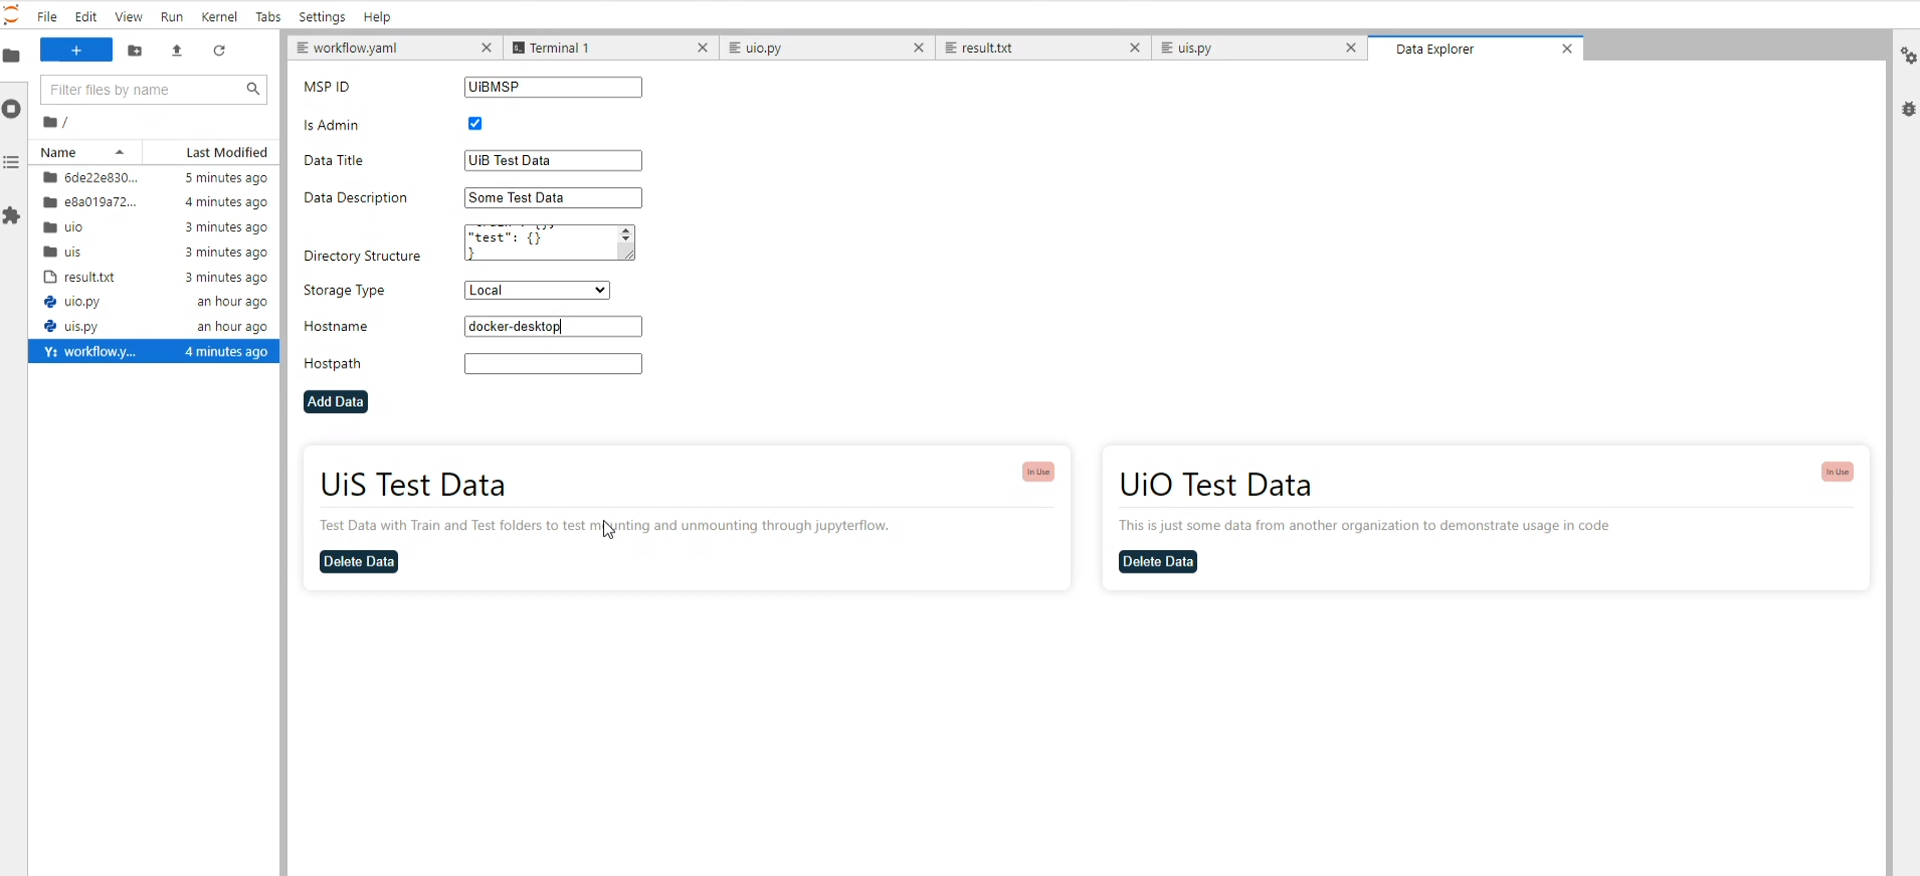
\includegraphics[width=14cm,keepaspectratio]{photos/Extension Screenshot.png}
    \caption{Screenshot of the extension in the proof of concept.}
    \label{fig:extension}
\end{figure}

\bigskip
Upon selection of a dataset for consumption, the extension creates a directory structure of the dataset in question with an id as the root of this directory structure. The user can write code experimenting with that directory structure. The extension also gets the decrypted sensitive information that can be used to mount the dataset and sets them in a hidden file on the File System. As mentioned before right now it is only secured by obscuring the information and hiding it from the user and can be improved upon in later work.

\subsection{JupyterFlow}
The last piece of the puzzle is JupyterFlow. It enables the users to run complex, compute-intensive workflows on a Kubernetes cluster while removing all the complexities of writing complicated YAML files for Argo and containerizing the code and the environment. 

\bigskip
We have extended the JupyterFlow to enable users to specify the volumes that a job in the workflow consumes and mount that volume before triggering the workflow. \ref{lst:basic-jflow} shows the basic YAML files that users could write to design complex workflows and JupyterFlow will convert it to the respective Argo Workflow and trigger it. \ref{lst:new-jflow} Is the YAML in our extended JupyterFlow plugin. The users can now specify the volumes as part of the jobs and these volumes will be mounted and consumed by that job only once the workflow is triggered. The id is received from the extension when a dataset is selected, the name can be a random name and the path is the path to mount the volume inside the container. 'dags' is the section describing workflow dependencies and the order to run the jobs in. The index starts at 1 for the first job, so the following workflow will run job 1 then after it has succeeded will run job 2 and job 3 in parallel.

\begin{lstlisting}[caption={YAML for mounting volumes using JupyterFlow in workflows in our custom JupyterFlow},label={lst:new-jflow}]
jobs:
- command: 'pwd' 
- command: 'ls -la /home/jovyan/uis'
  volumes:
  - id: ''
    name: ''
    path: ''
- command: 'ls'

dags:
- 1 >> 2
- 1 >> 3
\end{lstlisting}
%!TEX root = ../thesis.tex

\chapter{Experiment}
\label{ch:eval}

\section{Usecases and Overview}
We take inspiration from a supply chain network to design the workflow that will allow organizations to share datasets and other organizations to consume them without exposing the data itself. We think of data as an asset comparable to a physical asset, and use a blockchain as a centralized ledger between organizations to lease the data back and forth. The use of blockchain ledger allows the organizations to maintain their ownership over their datasets without trusting a third party maintaining the system, while others could lease and use the data to perform some analytics.

\bigskip
To test the system we design two main experiments to demonstrate the two different sources where data could be stored to be consumed by this proof of concept and also to demonstrate linear and parallel workflow design. In the next section, we will demonstrate how we can deploy the system and set it up for testing. Most of the same procedure can be used to set it up on VMs to set up a production environment. And finally, we will discuss the following two scenarios and how their workflow files are constructed and data sources for tests:

\begin{itemize}
    \item The workflow is linear and the data is hosted on a Kubernetes node.
    \item The workflow is parallel and results are combined and also the data for these parallel jobs are sourced in Azure File Shares.
\end{itemize}

\section{Deploy the System and Setup}
As \ref{fig:overview} highlights we have a couple of components that need to intercommunicate. So we will divide this deployment into two sections. In section one we discuss the deployment of the Hyperledger Fabric network and the REST API on a machine. And in the next section, we discuss building and deploying a JupyterHub server on a Kubernetes cluster. 

\subsection{Deploy Hyperledger Fabric}
In a production-ready system, each organization will set up Hyperledger on their own machines or nodes and join them to a network. We have already discussed the steps to join peers in a network. For the test here we use Docker to spin up nodes belonging to different organizations. We spin up a network with two participating organizations and a third orderer organization. And as the next step, we add a third participant organization or the fourth organization in total to this network. The docker-compose setup also starts certified authorities for the organizations.

\bigskip
It is recommended to run this on a machine separate from the Kubernetes cluster and accessible on a public IP since the project is configured to call a hard-coded IP from the browser and a Kubernetes headless service with the same IP. The pre requisites for the setup are Docker, Docker Compose, NodeJS, and NPM for the REST API. Following are the outlined steps to spin up and start a Hyperledger Fabric network with the chaincode and a REST API with Redis Cache and MySQL database on a machine using docker.

\begin{enumerate}
    \item SSH into the machine and get a shell session into the machine.
    
    \item Clone the repository for this thesis. \url{https://github.com/aliakbarrehman/master-thesis-uis}
    \begin{lstlisting}[language=bash]
    git clone https://github.com/aliakbarrehman/jupyterflow && cd master-thesis-uis\end{lstlisting}
    
    \item Run the following commands. The Script installs the Pre-Requisites as well as spins up the network with keys in \lstinline{hyperledger-network/crypto-config}, installs the chaincode for all organizations and spins up Rest API as well as Redis Cache and MySQL database.
    \begin{lstlisting}[language=bash]
    chmod +x spinUpNetwork.sh
    sudo ./spinUpNetwork.sh\end{lstlisting} 
\end{enumerate}

After the script finishes running the containers for certificates authorities, peers and chaincode containers for all organizations and orderer organizations along with the API, Redis and MySQL containers should be up. If the script run successfully \lstinline{docker ps} should show the output as in \ref{fig:vm-containers}

\begin{figure}
    \centering
    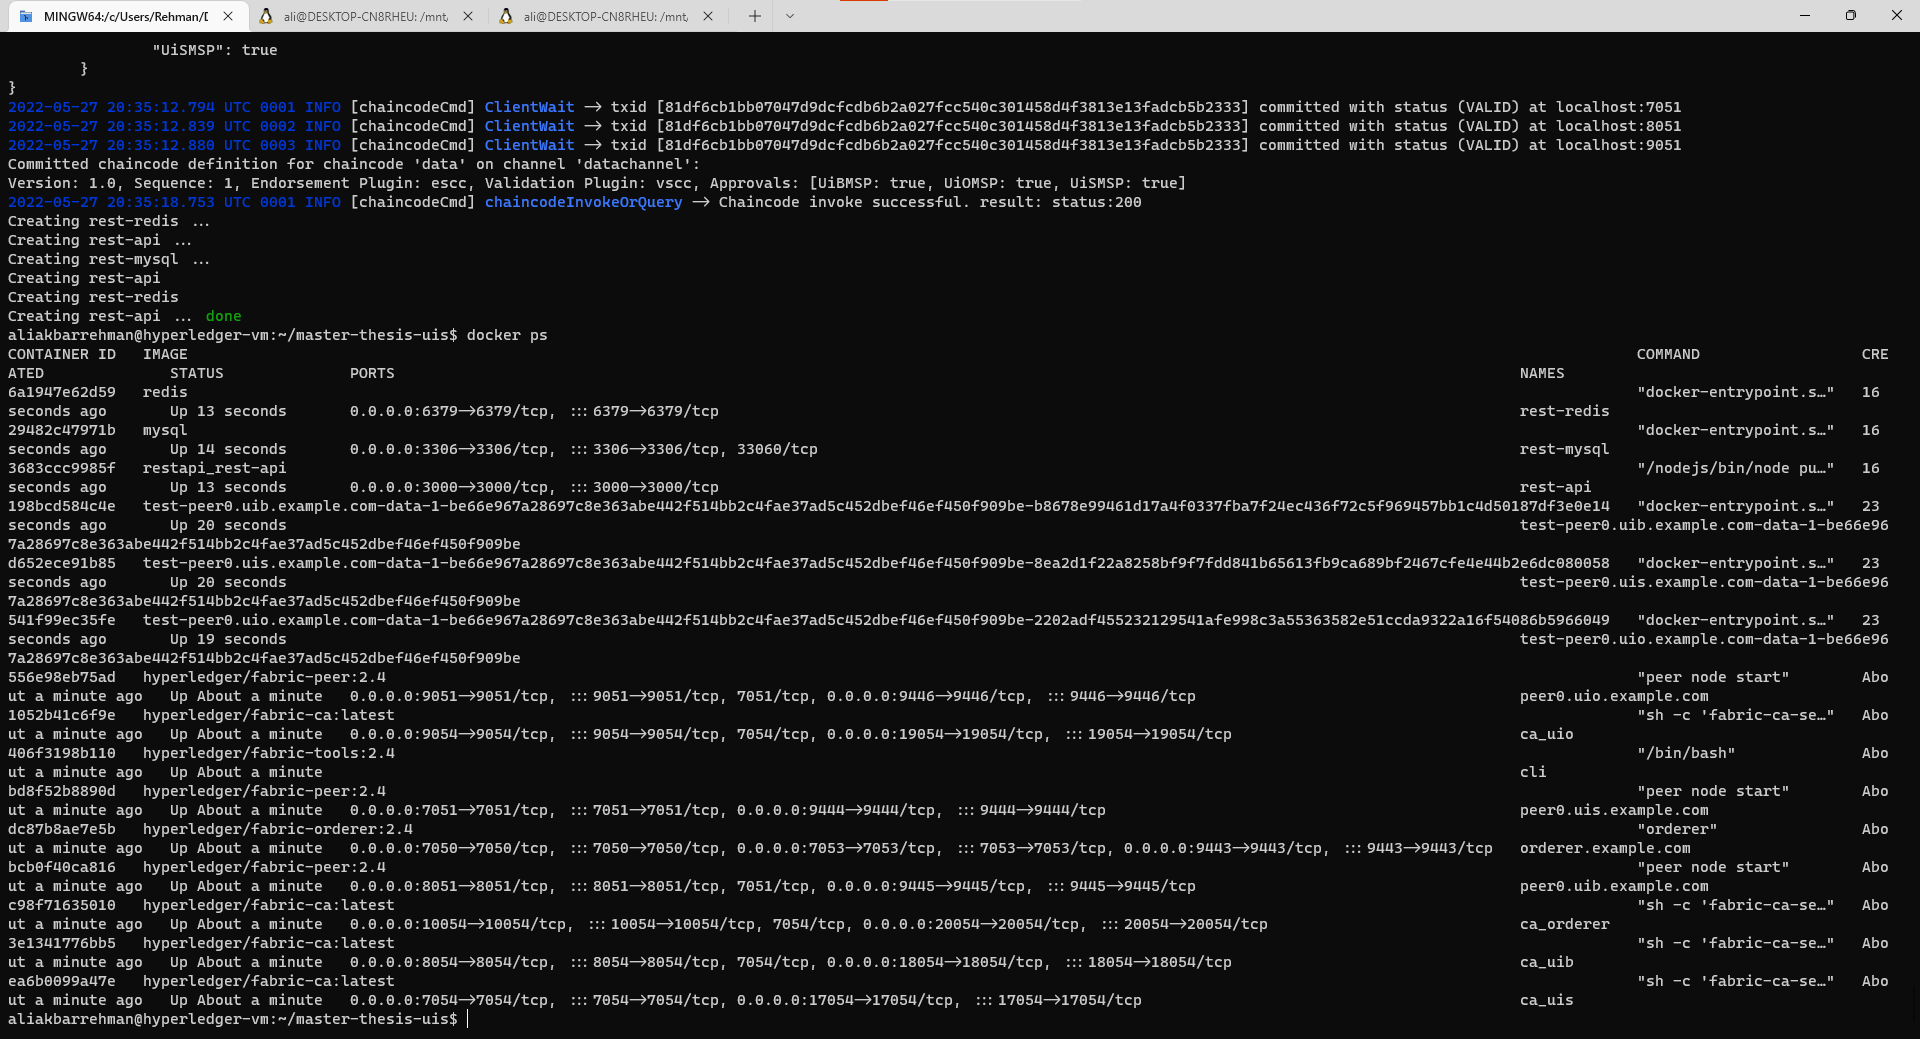
\includegraphics[width=14cm,keepaspectratio]{photos/Hyperledger-vm.png}
    \caption{The containers running on the Hyperledger VM after running the \lstinline{spinUpNetwork.sh} script successfully}
    \label{fig:vm-containers}
\end{figure}

\subsection{Deploy JupyterHub on Kubernetes}
The next component to set up for the demo is JupyterHub on Kubernetes. The pre requisites are Docker, NodeJS, NPM, Python, PIP, Kubernetes, and helm. The pre-requisites need to be installed following their respective setup instructions. Refer to the links in the footnotes for individual instructions.
\footnote{\url{https://docs.docker.com/engine/install/ubuntu/}}
\footnote{\url{https://github.com/nodesource/distributions/blob/master/README.md}}
\footnote{\url{https://linuxize.com/post/how-to-install-pip-on-ubuntu-20.04/}}
\footnote{\url{https://microk8s.io/\#install-microk8s}}

\begin{enumerate}
    \item Clone the repository for this thesis. \url{https://github.com/aliakbarrehman/master-thesis-uis}
    \begin{lstlisting}[language=bash]
    git clone https://github.com/aliakbarrehman/jupyterflow && cd master-thesis-uis\end{lstlisting}
    
    \item Change IP in \lstinline{jupyterhub/extension/thesis_extension/src/utils/api.ts} and
    \lstinline{jupyterhub/blockchain-service.yaml} with the public IP of the Hyperledger network as obtained from the previous section setup.
    
    \item Create a docker registry account and login to it \lstinline{docker login hub.docker.com}
    
    \item The first step to set up JupyterHub on Kubernetes is to build the extension and JupyterFlow into pip packages and build a docker image that will be used to spin up Jupyter Server for each user that logs in. We can run the \lstinline{buildJupyterhub.sh} with your docker hub repository.
    \begin{lstlisting}[language=bash]
    chmod +x jupyterhub/*.sh
    ./buildJupyterhub.sh aliakbarrehman/jupyterhub\end{lstlisting} 
    
    \begin{itemize}
        \item This script first creates a Kubernetes service account with permissions to manage secrets, persistent volumes, and persistent volume claims.
        \item Next it packages extension from \lstinline{jupyterhub/extension/thesis_extension}, extracts the wheel package name and copies it into docker context.
        \item Next the script packages our developed JupyterFlow from \lstinline{jupyterhub/jupyterflow}, extracts the wheel package name, and copies it into docker context.
        \item And finally the script builds a docker image with the extension and JupyterFlow installed and configured and the service account token set in environment variables. 
    \end{itemize} 
    
    \item Change \lstinline{singleuser.image.name} and \lstinline{singleuser.image.tag} in \lstinline{jupyterhub/config.yaml} with your own.
    
    \item Run \lstinline{./runJupyterhub.sh}. This script installs the JupyterHub from the helm charts, and the Argo workflow from helm charts, creates the load balancing services and creates roles, and binds them to the Argo workflow.
\end{enumerate}

\bigskip
Finally, once both the systems have been deployed, JupyterHub should be accessible on port 80 (\url{http://localhost}) and the Argo Workflow dashboard should be accessible at port 2746 (\url{https://localhost:2746}). And now users can log in to the JupyterHub and use the extensions to explore datasets, write code to consume datasets and trigger workflows that can be monitored on the Argo dashboard.

\section{Experiments}
\subsection{Linear Workflow with Local Dataset}
In the first experiment, we create two blocks on the blockchain for local datasets. By local here we mean datasets on the Kubernetes node. The workflow is linear where each job is run after the previous job has succeeded. The workflow for this example is presented in the listing \ref{lst:simple-wflow} The Ids are received when the user clicks to use a data.

\begin{lstlisting}[language=python,caption={Simple linear workflow.yaml consuming data from the Kubernetes node},label={lst:simple-wflow}]
jobs:
- command: 'ls /home/jovyan/'
- command: 'ls /home/jovyan/uis > result.txt'
  volumes:
  - id: '6de22e830ce4661cbeb6b9b2167c3f206dd946eb89beecd2f20bb17e85e64995'
    name: 'uis'
    path: '/home/jovyan/uis'
- command: 'ls /home/jovyan/uio >> result.txt'
  volumes:
  - id: 'e8a019a72cd8da522f620ab5561f5ada0143ea136ef71d8e601f6007c9386269'
    name: 'uio'
    path: '/home/jovyan/uio'

# Job index starts at 1.
dags:
- 1 >> 2
- 2 >> 3
\end{lstlisting}

When JupyterFlow is triggered with the command \lstinline{jupyterflow run -f workflow.yaml}, it mounts the data at \lstinline{/home/jovyan/uis} and \lstinline{/home/jovyan/uio} respectively. As dags (Directed Acyclic Graphs section) of the workflow state, the workflow is linear. It generates the Argo workflow as shown in \ref{fig:linear-wflow}

\begin{figure}
    \centering
    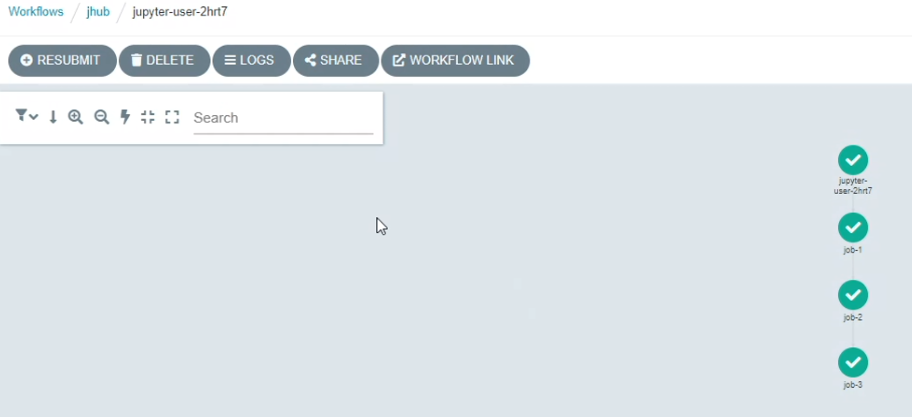
\includegraphics[width=10cm,keepaspectratio]{photos/linear-wflow.png}
    \caption{Linear workflow generated by the YAML file shown in listing \ref{lst:simple-wflow}}
    \label{fig:linear-wflow}
\end{figure}

\subsection{Complex Workflow with Azure and Local Datasets}

\begin{figure}
    \centering
    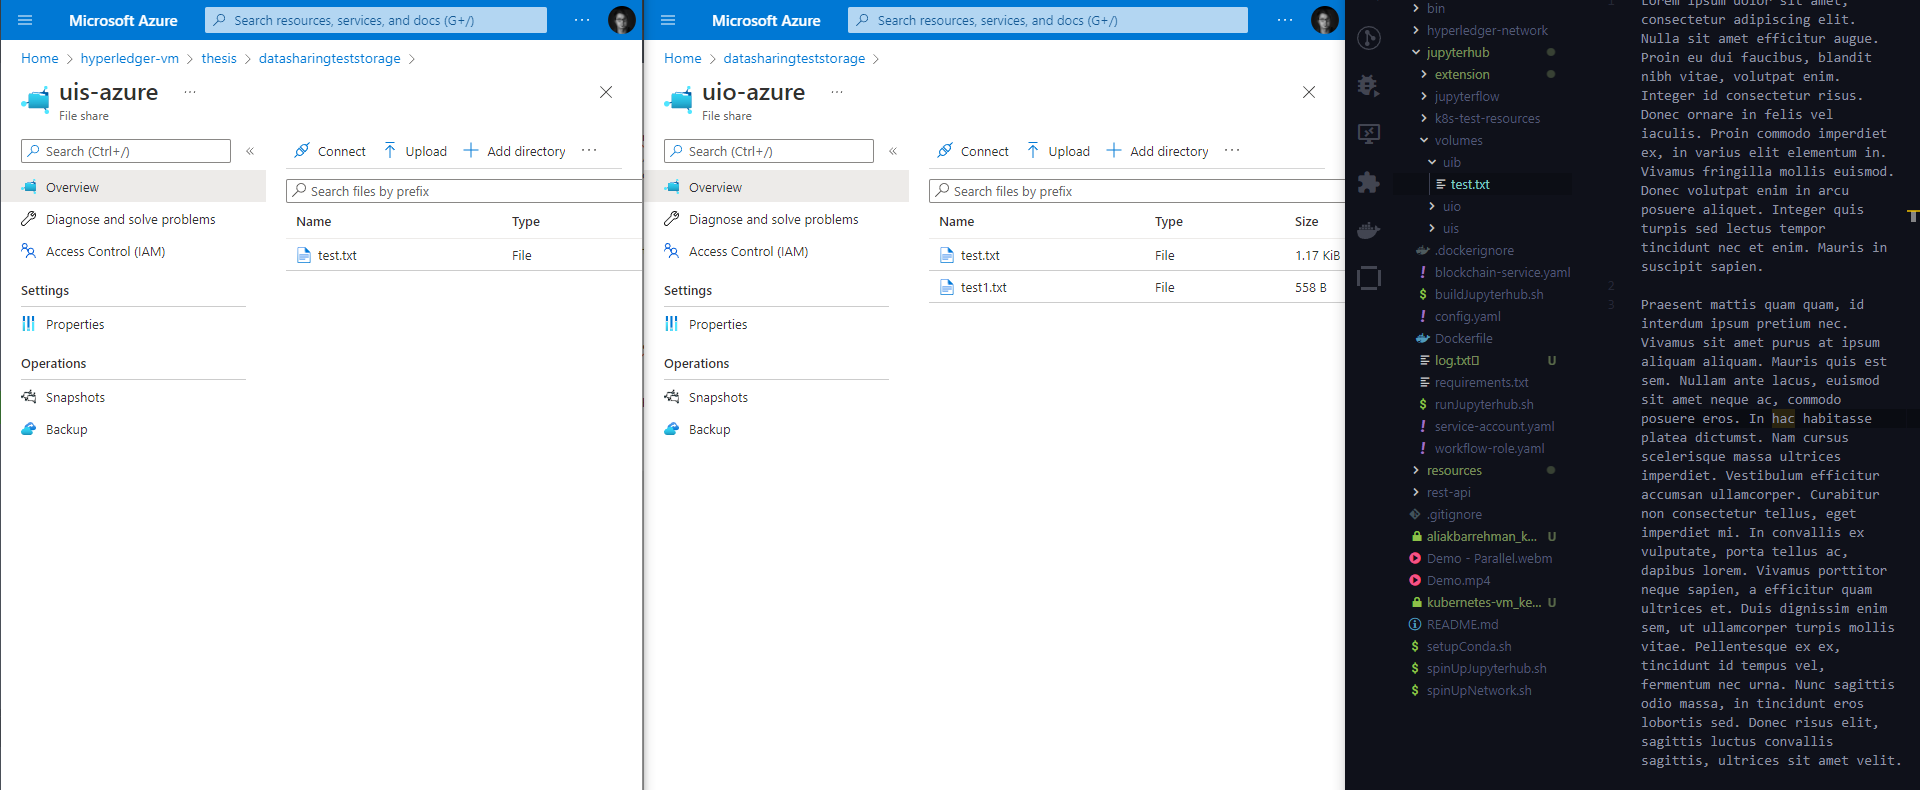
\includegraphics[width=14cm,keepaspectratio]{photos/dataset.png}
    \caption{Datasets for the complex workflow example. Azure File Shares and local dataset shown in VSCode}
    \label{fig:datasets}
\end{figure}

In the second experiment, we design and run a complex workflow that runs jobs in parallel and combines the results from them in the last job. Moreover, each job consumes data from different data sources. Two datasets are hosted in an Azure Storage Account in two different File Shares and the dataset for one job is hosted on the Kubernetes node itself.

\bigskip
In this experiment, we have the data hosted in azure and locally on the Kubernetes node as shown in the \ref{fig:datasets} datasets for UiO and UiS are in Azure and UiB hosted their data on the Kubernetes node. UiO, UiS, and UiB are test organizations and we have no formal dataset agreement for this demo.

\bigskip
The listing \ref{lst:parallel-wflow} shows the workflow.yaml for this experiment that JupyterFlow consumes. Dags section here sets up the workflow to run parallel jobs. And the last job combines and outputs the result of the workflow. The Ids are received when the user clicks to use data. This produces the \ref{fig:parallel-wflow} workflow in Argo.

\begin{lstlisting}[caption={Complex workflow consuming data from Azure},label={lst:parallel-wflow}]
jobs:
- command: 'ls /home/jovyan/'
- command: 'python uis.py'
  volumes:
  - id: '36b0c4d057e1bf9c0915e66330d18299d0f08c0c0f0340847cc879b3fbf73b4d'
    name: 'uis'
    path: '/home/jovyan/uis'
- command: 'python uio.py'
  volumes:
  - id: 'c12e28fb1d8c4bb243d5e7622afd90fde92ddb53971be384b92c33a464c80451'
    name: 'uio'
    path: '/home/jovyan/uio'
- command: 'python uib.py'
  volumes:
  - id: '3011ffd02613bb0971fb14b3bcbfea54ab1141afcd78c06ca18337f29740abbc'
    name: 'uib'
    path: '/home/jovyan/uib'
- command: 'python final-result.py'

dags:
- 1 >> 2
- 1 >> 3
- 1 >> 4
- 2 >> 5
- 3 >> 5
- 4 >> 5
\end{lstlisting}

\begin{figure}
    \centering
    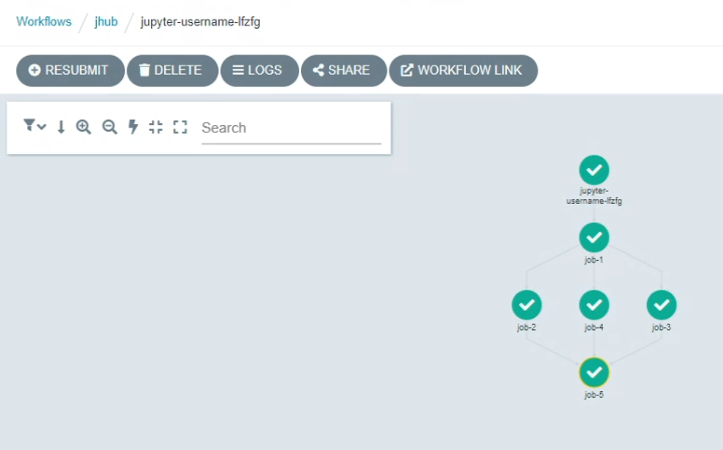
\includegraphics[width=10cm,keepaspectratio]{photos/parallel-wflow.png}
    \caption{Parallel Workflow generated by the YAML file shown in listing \ref{lst:parallel-wflow}}
    \label{fig:parallel-wflow}
\end{figure}

\bigskip
The listings \ref{lst:uis-py} and \ref{lst:final-result-py} show the python code that is run for each job in the complex workflow. The code counts the occurrences of work \textbf{lorem} in files under a dataset. And the \lstinline{final-result.py} has code that aggregates and outputs the final results to a file.

\begin{lstlisting}[language=python,caption={uis.py similar to uio.py and uib.py. The code that is run for the parallel jobs},label={lst:uis-py}]
import os

path = '/home/jovyan/uis'
files = []
for (dirpath, dirnames, filenames) in os.walk(path):
    for i in filenames:
        files.append(os.path.join(dirpath, i))
    break
    
count = 0
for i in files:
    f = open(i, 'r')
    for line in f:
        count += line.count('lorem')

f = open('/home/jovyan/uis-count.txt', 'a')
f.write('UiS: ' + str(count) + '\n')
f.close()
\end{lstlisting}

\bigskip

\begin{lstlisting}[language=python,caption={final-result.py that combines the output of the parallel jobs and computes the output},label={lst:final-result-py}]
import os

path = '/home/jovyan/uis'
files = ['uis-count.txt', 'uio-count.txt', 'uib-count.txt']

result = ''
for i in files:
    f = open(i, 'r')
    for line in f:
        result += line + '\n'

f = open('/home/jovyan/result.txt', 'a')
f.write(result)
f.close()
\end{lstlisting}

A complete demonstration of the experiments can be found at \url{https://github.com/aliakbarrehman/master-thesis-uis/blob/master/Demo\%20-\%20Parallel.webm} and \url{https://github.com/aliakbarrehman/master-thesis-uis/blob/master/Demo.mp4}
%!TEX root = ../thesis.tex

\chapter{Conclusions and Future Work}
\label{ch:conclusion}
In this thesis, we present a Proof of Concept (PoC) that allows data sharing between untrusting organizations to run complex workflows on the data while also maintaining the ownership of the data. Another goal achieved from such a system is that we remove the need to develop the expertise of users to write complex algorithms following the Hadoop MapReduce pattern.

\bigskip
We go through the scenarios that could benefit from such a system and some background about research in this direction as well as tools and technologies we have used. We have proposed a solution to allow data sharing and workflow execution. The proposed system makes use of Hyperledger Fabric to establish and maintain a blockchain between organizations and JupyterHub on Kubernetes for users to write code and run workflows. We build a Docker image with Kubernetes service account configured and JupyterHub Extension and JupyterFlow already installed on it and use the said image for JupyterHub. Each logged-in user gets their own instance of Jupyter hosted on the Kubernetes server. And after writing code and triggering workflow, the data is mounted as persistent volumes on the Kubernetes pods where it is used. And finally, we demonstrate how we set up our test environments and ran linear and parallel workflows on the system, consuming data from Azure and Kubernetes nodes.

\bigskip
The system is far from a production-ready system and can be improved upon in many different aspects regarding security and capabilities. Next up we discuss the shortcomings in our system and the future directions for the thesis and how the research in this domain can be carried forward.

\section{Integration with Relevant Projects}
As mentioned in the chapter on introduction, this proof of concept is being developed in parallel to a few other projects aimed toward a solution with access control and motivating organizations to make and join such consortiums. As demonstrated in \ref{fig:overview} the scope of this thesis was to design and test a system that can be used to orchestrate all the moving parts and enable users to explore the datasets from the blockchain and consume the said datasets for analytics.

\bigskip
During this thesis, we have been using test accounts to log into the JupyterHub server. Moreover, for interaction with the blockchain the REST API sets up a file system wallet to identify the users when invoking chaincode. There is a thesis that is aiming to develop a distributed identity token system that maintains the users and their access control on the blockchain itself. As the next natural step to take this proof of concept further is to integrate it with the aforementioned project. That will allow not only this system users to log in to JupyterHub with this but also remove the need for each organization to maintain their respective wallets.

\bigskip
\cite{nft-thesis} Is developing a system that represents resources as a token with stakes of different organizations in the token. If we integrate this solution into our proof of concept, we can store the computed results onto the blockchain and Inter-Planetary File System (IPFS) as well, and anytime the results are used we can incentivize the organizations with a stake in that token to motivate organizations to contribute. Moreover, we can take inspiration to use IPFS to store metadata of the datasets instead of storing it directly on the blockchain and peer nodes.

\section{Secure Transfer of Storage Secrets}
In the current implementation once the user elects to use a dataset the JupyterHub extension that we have developed does a couple of steps to ensure its usage.
\begin{itemize}
    \item First of all the extension submits a transaction to the blockchain to lease the dataset, so as to avoid others leasing it at the same time causing conflicts.
    \item After the transaction, the extension reads decrypted values of sensitive information that will be used to mount the actual data inside Kubernetes.
    \item Now the extension creates a directory structure in the JupyterHub environment for the user to write the code following that directory structure and avoid errors when running the workflow.
    \item As a final step the extension creates a hidden file in the environment with the sensitive information that can be used to mount the data as volume. The JupyterFlow plugin uses this hidden file to mount the data onto Kubernetes before triggering the Argo workflow.
\end{itemize}

As apparent from the last step mentioned above, the security we have at the moment is only security by obscurity and is very easy to bypass because the user can view the hidden files very easily either through the terminal in the Jupyter Instance of or through python code. The security regarding this can be improved upon a lot and the flow of information from the extension to the JupyterFlow plugin can be improved and made secure. Either by limiting users to not being able to access the file or by developing a protocol for the transfer of information directly between these components instead of using the file system. 

\section{Clean Up of Resources}
When the user elects to consume a dataset and after the execution of the workflow finishes the volume claim in Kubernetes needs to be released and volume to be deleted. Moreover, a transaction should be submitted to the blockchain notifying the release of the resource so as another organization may use that data.

\bigskip
Also, there could be the need to do a few more steps such as computing the result NFT and committing it to the chain when the computation has finished when integrating with \cite{nft-thesis}.

\bigskip
The next iteration of this proof of concept could leverage exit handlers \cite{argo-exit-handler} provided by Argo to trigger an HTTP endpoint that can perform all the above-mentioned steps and cleans up the resources or could use a shell script to clean up. That if triggering a shell script the workflow role created for Argo would need privileges to clean up the resources from Kubernetes. It does not need access to create or update the Persistent Volume and Persistent Volume Claim objects but rather just the permissions to delete these objects.

\bigskip
And to avoid users running a workflow that never finishes the keeps the dataset occupied for a longer period of time we should introduce a scheduled trigger to force the release of the resources.

\section{Extending Capabilities of JupyterFlow}
Apart from changing the patterns to improve security and implementing cleanup of resources the capabilities of the JupyterFlow plugin could be improved upon more. We could integrate more and more storage solutions into the system. So that the next phase of the thesis would support the mounting of Google Cloud Storage, Amazon S3 Buckets, Network File Systems, and many more.

%-----------------------------------------------------------------
% Now begin the Appendices, including them as separate files

\listoffigures
\lstlistoflistings

\appendix
%!TEX root = ../thesis.tex

\chapter{Code and Instructions}
\label{apx:instructions}

The GitHub Repository with the code and resources for this thesis can be found at \url{https://github.com/aliakbarrehman/master-thesis-uis}.

\bigskip
The code has the following directories:
\begin{itemize}
    \item \textbf{bin} This directory has the binaries for the Hyperledger Fabric commands. This is included in the repository to make this self-hosted without external dependencies to download and set up.
    \item \textbf{hyperledger-network} The directory holds the configuration files, docker-compose files, chaincode, and scripts to spin up the network, add organizations and commit chaincode to the network.
    \item \textbf{jupyterhub} This directory hosts everything JupyterHub-related. The root directory hosts the scripts, and configurations to build the image for JuptyerHub Kubernetes, and create the required service accounts and scripts to spin up the Kubernetes itself with JuptyerHub and Argo enabled.
        \begin{itemize}
            \item \textbf{extension} The directory contains the code for the extension for JupyterHub that enables exploration of datasets stored on the blockchain.
            \item \textbf{jupyterflow} This directory hosts the code for the JupyterFlow plugin.
        \end{itemize}
    \item \textbf{resources} Resources directory has the architecture diagrams and endpoint information and examples.
    \item \textbf{rest-api} REST API that interacts with the blockchain.
\end{itemize}

The video demo can be found in the repository as well.

\section{Instructions}
Following are the instructions to setup the project for testing.
\begin{itemize}
    \item Get a machine with a public IP that k8s cluster can call, Pre-Requisites Docker, Docker Compose, NodeJS and NPM.
    \item SSH into the machine
    \item Clone this repository \lstinline{git clone https://github.com/aliakbarrehman/jupyterflow && cd master-thesis-uis}
    \item Run \lstinline{chmod +x spinUpNetwork.sh && ./spinUpNetwork.sh} that Installs the Pre-Reqs as well as spins up the network with keys in \lstinline{hyperledger-network/crypto-config} and spins up Rest API as well as REDIS Cache and MySQL DB
    \item Alternatively for more granular control you can install requirements and run \lstinline{cd hyperledger-network && ./start.sh}
    \item Run \lstinline{./start.network.sh}
    \item Run \lstinline{cd ../rest-api and then docker-compose up -d}
    \item For testing import \lstinline{resource/endpoints.json} into postman and create some datablocks on blockchain
    \item On another machine. Pre-Requisites Docker, NodeJS, NPM, Python, PIP, Kubernetes and helm
    \item Clone this repository \lstinline{git clone https://github.com/aliakbarrehman/jupyterflow && cd master-thesis-uis}

    \item Change directory to jupyterhub \lstinline{cd jupyterhub}

    \item Create a docker registry account and login to it docker \lstinline{login hub.docker.com}

    \item Run with your own registry name e.g \lstinline{./buildJupyterhub aliakbarrehman/jupyterhub}. This script creates a k8s service account, packages extension from \lstinline{jupyterhub/extension/thesis_extension} (Some useful commands in \lstinline{extension/usefulCommandsForDevelopment.sh} for development), packages extension from \lstinline{jupyterhub/jupyterflow} and builds a docker image with all the previous packages installed and configured (This image will be used for spinning up a users notebooks / JupyterHub instances and pushes that image)

    \item Change \lstinline{singleuser.image.name} and \lstinline{singleuser.image.tag} in \lstinline{jupyterhub/config.yaml} with your own

    \item Change IP in \lstinline{jupyterhub/blockchain-service.yaml} with the public IP of the Hyperledger network

    \item Change IP in \lstinline{jupyterhub/extension/thesis_extension/src/utils/api.ts} with the public IP of the Hyperledger  network

    \item Run \lstinline{./runJupyterhub.sh}
\end{itemize}
Jupyterhub can be accessed at http://localhost and Argo can be accessed at localhost:2746. After logging into Jupyterhub (for testing you can use user as username and password as password). Explore datasets available on DataExplorer. Use it by writing code and workflow.yaml and running the workflow as described above. View the workflow status on Argo at https://localhost:2746/workflows
%-----------------------------------------------------------------
% \backmatter

% \label{Bibliography}
% \bibliographystyle{unsrtnat}  % Use the "unsrtnat" BibTeX style for formatting the Bibliography
% \bibliography{Bibliography}  % The references (bibliography) information are stored in the file named "Bibliography.bib"
\printbibliography
\uisbackcover
\end{document}
